\documentclass[11pt,leqno,oneside]{amsbook}
\usepackage{tikz}
\usetikzlibrary{cd}
\usepackage{bbm}
\usepackage{ytableau}
\usepackage{todonotes}

\usepackage{../notes}
\usepackage{../../ReAdTeX/readtex-core}
\usepackage{../../ReAdTeX/readtex-abstract-algebra}
\usepackage{../../ReAdTeX/readtex-lie-algebras}

\numberwithin{thm}{section}

\newcommand{\bbk}{\mathbbm{k}} % base field
\newcommand{\Rep}{\operatorname{Rep}} % category of representations
\renewcommand{\Q}{Q} % quiver
\newcommand{\grdim}{\boldsymbol{\dim}} % graded dimension
\newcommand{\gr}{\operatorname{gr}} % graded representation
\newcommand{\sinktosource}{s^\downarrow} % reflection from sink to
% source
\newcommand{\sourcetosink}{s^\uparrow} % reflection from source to sink
\newcommand{\sinksource}{s^{\uparrow \downarrow}} % shorthand for both
\newcommand{\sinktosourcefunc}{\Phi^\downarrow} % BGP reflection functor
\newcommand{\sourcetosinkfunc}{\Phi^\uparrow} % BGP reflection functor
\newcommand{\sinksourcefunc}{\Phi^{\downarrow \uparrow}} % Shorthand
                                % for both functors
\newcommand{\subtableau}{\normsubgroup}
\newcommand{\SymF}{\Lambda} % ring of symmetric functions
\newcommand{\cF}{\mathcal{F}} % Hall algebra set
\newcommand{\quantumBinom}[3][q]{\left[ \begin{array}{c} #2 \\
                                          #3 \end{array} \right]_#1}
\newcommand{\Gr}{\operatorname{Gr}} % Grassmanian
\newcommand\mapsfrom{\mathrel{\reflectbox{\ensuremath{\mapsto}}}}

\newcommand{\roots}{R} % Root System. This symbol may change later
\newcommand{\bbQ}{\mathbb{Q}} % For rationals since \Q is for quiver now
\newcommand{\A}{\tilde{\mathcal{A}}} 
\newcommand{\U}{U}

\title[Geometric Representation Theory]{Geometric Representation
  Theory: Lecture notes from a class taught by Weiqiang Wang}
\author{George H. Seelinger}
\date{Fall 2017}
\begin{document}
\maketitle
\section{Quivers and Quiver Algebras}
\subsection*{(8/22/2017) Lecture 1}
This class will cover some topics in geometric representation
theory. Our general outline is
\begin{enumerate}
\item[(1)] Quiver representations, including Dynkin quivers and Gabriel's
  classification of indecomposables.
  \begin{itemize}
  \item Non-simply laced [Geiss, Lederc, Schr\"{o}er] (arXiv 1410.1403)
  \item ``Affine'' (Euclidean) quivers
  \end{itemize}
\item[(2)] Hall algebras, including ``classical'' Hall algebras which leads
  to Hall-Littlewood polynomials, and Ringel (over \(\F_q\)), which
  has connections to half quantum groups.
\item[(2.5)] Springer theory. This will be covered in a reading course
  and not included here. However, convolution algebra on ``Steinberg
  varieties'' leads to Weyl groups and representations.
\item[(3)] Quiver varieties. From this and the above, we get the
  Lusztig (semi)canonical basis, which leads to Nakajima's work on
  integrable modules of Kac-Moody semisimple Lie algebras. Type A is
  covered in Chriss-Ginzburg, chapter 4.
\end{enumerate}
\begin{defn}
  A \de{quiver} is a tuple \(\Q = (I,\Omega,s,t)\) (sometimes denoted
  \((\Q_0,\Q_1,s,t)\)) where \(I\) is the vertex set, \(\Omega\) is the
  edge set, and \(s,t \from \Omega \to I\) such that, for \(h \in
  \Omega\), \(h \mapsto s(h), t(h)\), respectively. We say \(h\)
  starts at \(s(h)\) and terminates at \(t(h)\). 
\end{defn}
\[
\begin{tikzcd}
s(h) \arrow[r,"h"] & t(h)
\end{tikzcd}
\]
\begin{defn}
  Given a quiver \(\Q\), we say \(\left| \Q \right|\) is the underlying
  graph with direction removed.
\end{defn}
Throughout these lecture notes, unless otherwise stated, we will
always assume \(\Q\) is connected and that we are working of ground
field \(\bbk\).
\begin{example} \label{ex1} Examples of small quivers include:
  \begin{enumerate}
  \item[(a)]  \[
      \begin{tikzcd}
        1 \arrow[out=0,in=90,loop]
      \end{tikzcd}
    \]
  \item[(b)] \[
      \begin{tikzcd}
        1 \arrow[r,""] & 2
      \end{tikzcd}
    \]
  \item[(b')] \[
      \begin{tikzcd}
        1 \arrow[r,""] & 2 \arrow[r] & 3
      \end{tikzcd}
    \]
  \item[(c)] \[
      \begin{tikzcd}
        1 \arrow[r,bend left,""] \arrow[r,bend right,swap,""] & 2
      \end{tikzcd}
    \]
  \end{enumerate}
\end{example}
\begin{defn}
  A \de{representation} of a quiver \(\Q\) consists of the data
  \begin{itemize}
  \item To each \(i \in I\), assign \(\bbk\)-vector space \(V_i\).
  \item To each \(h \in \Omega\), assign a linear map \(x_h \from
    V_{s(h)} \to V_{t(h)}\)
  \end{itemize}
\end{defn}
\begin{defn}
  A \de{morphism of representations} \(f \from V \to W\) consists of
  linear maps \(f_i \from V_i \to W_i\) and makes the following
  diagram commute.
\[  \begin{tikzcd}
    V_{s(h)} \arrow[d, "f_{s(h)}"] \arrow[r,"x_h"] & V_{t(h)} \arrow[d, "f_{t(h)}"] \\
    W_{s(h)} \arrow[r,"y_h"] & W_{t(h)}
  \end{tikzcd}
\]
\end{defn}
\begin{defn}
  Given representations \(V,W\), we define \(\Hom(V,W) = \Hom_\Q(V,W)\) as the set of all morphisms
  from \(V,W\). We also let \(\Aut_Q(V)\) be all invertible morphisms
  in \(\Hom(V,V)\).
\end{defn}
We will denote the category of (not necessarily finite-dimensional)
representations of \(\Q\) as \(\Rep(\Q)\). A basic problem of this
course is to classify (simple, indecomposable) representations of
\(\Q\), up to isomorphism.
\begin{example}
  \begin{enumerate}
  \item Consider \ref{ex1}(a). This is the same as asking the classification
  of all \(f \from \bbk^n \to \bbk^n\). If \(\bbk = \C\), then this is
  well-known by the Jordan canonical form for square matrices.
  \item Consider \ref{ex1}(b) and assign \(V_1\) to vertex 1 and
    \(V_2\) to vertex 2. Then, if\(x \from V_1 \to V_2\) has rank
    \(r\), it is of the form, up to a
    change of basis for \(V_1\) and \(V_2\), \[
      x \approx \left(
        \begin{array}{cc}
          I_{r \times r}& 0 \\
          0 & 0
        \end{array}
      \right)
    \]
  \end{enumerate}
\end{example}
Remember that we can make sense of subrepresentations and quotient
representations of \(\Q\).
\begin{thm}
  \(\Rep(\Q)\) is closed under \(\bigoplus\), taking
  kernel/cokernel, and subreprresentations and quotients. That is, \((\ker f)_i := \ker(f_i \from V_i \to
  W_i)\). Hence, \(\Rep(\Q)\) is an abelian category.
\end{thm}
\begin{proof}
  We must show that \(\ker f\) is actually a representation. If
  \(v \in (\ker f)_{s(h)}\), then \((f_{t(h)} \circ x_h)(v) = (y_h \circ
  f_{s(h)})(v) = 0\) by the definition of a representation morphism
  and the fact that \(v\) is in the kernel of \(f_{s(h)}\). Thus
  \(x_h(v) \in (\ker f)_{t(h)}\) and \(x_h\) induces a map from
  \((\ker f)_{s(h)} \to (\ker f)_{t(h)}\). We can apply a similar
  argument for cokernel. \\

  If we define \(\oplus\) in the obvious way, \((V \oplus W)_i = V_i
  \oplus W_i\), we get a direct sum representation. 
\end{proof}
\begin{defn}
  A \de{path} in a quiver \(\Q\) (of length \(\ell\)) is a series of
  edges in \(\Q\), say \((h_1, \ldots, h_\ell)\) such that \(t(h_i) =
  s(h_{i+1})\) for all \(i\). We denote such a path as \(h_\ell \cdots
  h_2 h_1 \from s(h_1) \to t(h_\ell)\). 
\end{defn}

\begin{defn}
  A \de{path algebra} \(\bbk \Q\) is given as the free module with
  basis given by paths in the quiver \(\Q\) endowed with a
  multiplication operator on basis elements \(f,g\) given by \[
    f \cdot g = \begin{cases}
      0 & t(g) \neq s(f) \\
      \begin{tikzcd}
        s(g) \arrow[r,"g"] & t(g) \arrow[r,"f"] & t(f)
      \end{tikzcd} & t(g) = s(f)
    \end{cases}
  \]
\end{defn}
\begin{defn}
  A \de{path of length 0} in a quiver \(\Q\) is of the form \(e_i\) for
  \(i \in I\). For \(p \in \bbk Q\), we say \[
      e_i \cdot p = 
    \begin{cases}
      p & t(p) = i \\
      0 & \text{ else }
    \end{cases} \ \ \ p \cdot e_i =
    \begin{cases}
      p & s(p) = i \\
      0 & \text{ else }
    \end{cases}
  \]
\end{defn}
\begin{prop}
  \(e_i\) is an orthogonal idempotent of \(\bbk \Q\).
\end{prop}
\begin{proof}
  Consider that \(e_i^2 = e_i\) and \(e_i e_j = 0\) for \(i \neq j\)
  by definition of \(e_i\). (Note, as stated, this is not actually true.)
\end{proof}
\begin{prop}
  \(\bbk \Q\) is associative with \(1 := \sum_{i \in I} e_i\). 
\end{prop}
\begin{prop}
  \(\bbk \Q\) is \(\Z_{\geq 0}\)-graded by path lengths.
\end{prop}
\begin{example}
  For quiver \(Q = (I,\Omega,s,t)\), we get \((\bbk Q)_0 =
  \bigoplus_{i \in I} \bbk e_i\) and \((\bbk Q)_1 = 
  \bigoplus_{h \in \Omega} \bbk h\).
\end{example}
\begin{prop}
  \(\bbk \Q\) is finite-dimensional if and only if \(\Q\) has no oriented cycles.
\end{prop}
\begin{proof}
  If \(\Q\) has an oriented cycle, then \(\bbk \Q\) may be
  infinite-dimensional. Consider \(\Q\) as \ref{ex1}(a). Then, \(\bbk
  Q\) is the algebra of all polynomials in 1 generator,
  \(\bbk[x]\). For the forwards direction, ...
\end{proof}
\begin{example}
  Consider the path algebra of \ref{ex1}(b). This algebra has
  dimension 3: 2 paths of length 0 and 1 path of length 1. Similarly,
  \ref{ex1}(b') has 3 paths of length 0, 2 paths of length 1, and 1
  path of length 2, giving us a total of 6 paths.
\end{example}
\begin{prop}\label{hom-of-Aei}
  Let \(A := \bbk Q\). Then, \[
    A = \bigoplus_{i \in I} A e_i
  \]
  and \(A e_i\) is a projective left \(A\)-module. Furthermore, given
  an \(A\)-module \(M\), we get \[
    \Hom_A(A e_i, M) \isom e_i M
  \]
\end{prop}
\begin{proof}
  The decomposition of \(A\) is a standard fact for primitive
  orthogonal idempotents of an algebra. \(A e_i\) is projective
  because it is a direct summand of the free \(A\)-module \(A\). \\

  To show the isomorphism, we first note that \(f \in \Hom_A(A e_i,
  M)\) is uniquely determined by \(f(e_i)\). This is because \(f\)
  must be \(A\)-linear, so \(f(a e_i) = a.f(e_i)\) for all \(a \in
  A\). Furthermore, \(f(e_i) \in e_i M\) because \(f(e_i) = f(e_i^2) =
  e_1.f(e_i)\). Thus, consider the \(A\)-module homomorphism given by
  \(\phi \from \Hom_A(A e_i, M) \to e_i M\) given by \(f \mapsto
  f(e_i)\). We already know that \(\phi\) is injective since, if
  \(\phi(f) = \phi(g)\), then \(f(e_i) = g(e_i) \implies f =
  g\). Furthermore, \(\phi\) is injective since, given \(e_i m \in e_i
  M\), there is an \(f \in \Hom(A e_i, M)\) such that \(f(e_i) = m\). 
\end{proof}
\begin{prop}
  Given \(0 \neq f \in A e_i\) and \(0 \neq g \in e_i A\), it must be
  that \(fg \neq 0\). This follows from the fact that \(fg\) must pass
  through \(i\) and has nonzero length. 
\end{prop}
\begin{prop}
  The \(e_i\)'s are \emph{primitive} idempotents, that is, \(A e_i\)
  is indecomposable.
\end{prop}
\begin{proof}
  We wish to show that the only idempotent in \(\End_A(A e_i)\) is
  \(e_i\) since, if \(Ae_i \isom M \oplus N\) for non-trivial \(M,N\), then \(A e_i \onto M
  \into A e_i \) would be an idempotent in \(\End_A(A e_i)\). By
  \ref{hom-of-Aei}, \(\End_A(A e_i) \isom e_i A e_i\). Take idempotent
  \(f \in e_i A e_i\). Then, \(f^2 = f = f e_i\), so \(f(f-e_i) = 0
  \implies f = e_i\) by the preceding proposition.
\end{proof}
\begin{prop}
  \(A e_i \not \isom A e_j\) as \(A\)-modules for \(i \neq j\)
\end{prop}
\begin{proof}
  If \(A e_i \isom A e_j\), then take \(f \in \Hom_A(A e_i, A e_j)
  \isom e_i A e_j\) (by previous proof) to be an isomorphism and \(g
  \in e_j A e_i\)
  to be its inverse. Then, \(fg = e_i \implies e_i \in A e_j A\). This
  is only possible when \(i = j\). 
\end{proof}
\begin{prop}
  \(\Rep(\Q) \isom \bbk Q\)-Mod.
\end{prop}
\begin{proof}
  Consider the map \((V_i)_{i \in I} \mapsto V = \bigoplus_{i \in
    I} V_i\) where \[
    h_\ell \cdots h_q \cdot v =
    \begin{cases}
      x_{h_\ell} \cdots x_{h_1} (v_i) & i = s(h_i) \\
      0 & \text{ else }
    \end{cases}
  \]
  This sends a representation \((V_i)\) to a \(\bbk \Q\)-module.  \\
  
  Conversely, given a \(\bbk \Q\)-module \(M\), we can construct an
  inverse to the map above by letting 
  \(M_i := e_i M\) and taking \(M = \bigoplus_{i \in I} e_i M\) and
  letting \(h \in \Omega\) be \(h \from M_{s(h)} \to M_{t(h)}\). We
  note that \(h(M_i) \subset M_j\), so the collection \((M_i)\)
  satisfies the definition of a representation of \(\Q\). 
\end{proof}
Due to this theorem, we will often use representations of \(\Q\) and
\(\bbk \Q\)-modules interchangably.
\subsection*{(8/24/2017) Lecture 2}
\begin{defn}
  Let \(\Q\) be a quiver. For \(i \in I\), we define the
  representation \[
    S(i) :=
    \begin{cases}
      \bbk & \text{ at }i \\
      0 & \text{ else }
    \end{cases}
  \]
\end{defn}
\begin{thm}
  If a quiver \(\Q\) has no oriented cycles, then \(\{S(i)\}_{i \in
    I}\) is a full list of simple \(\bbk \Q\)-modules. 
\end{thm}
\begin{proof}[Proof by Example]
  Let \(V\) be a simple representation of quiver \[
    \begin{tikzcd}
      1 \arrow[r] & 2
    \end{tikzcd}
  \]
  with \(V_1 \neq 0 \neq V_2\). Then, consider the inclusion of the
  representation given below.
  \[
    \begin{tikzcd}
      0 \arrow[r] \arrow[d] &  V_2 \arrow[d] & = e_2 V  \\
      V_1 \arrow[r] & V_2 &
    \end{tikzcd}
  \]
  Because there are no edges starting from \(2\), there can be no
  non-zero map starting at \(V_2\) in \(V\), so we have found a
  sub-representation of \(V\), which is a contradiction. The full
  proof is of the same spirit, but replace 1 and 2 with \(i\) and
  \(j\) where, since \(\Q\) is acyclic, there is a \(j\) such that no
  edges start at \(j\). 
\end{proof}
\begin{defn}
  Let \(A = \bbk \Q\). Then, we define \[
    P(i) := A e_i
  \]
  which is projective, as noted earlier.
\end{defn}
Since \(P(i)\) consists of all paths starting at \(i\), then, if there
is an edge going from \(i\) to \(j\), \(P(i)\) has a submodule
isomorphic to \(P(j)\).
\begin{prop}
  For an acyclic quiver \(\Q\), we get \(P(i)/\operatorname{rad} P(i)
  \isom \operatorname{hd}(P(i)) \isom S(i)\) where
  \(\operatorname{rad} P(i)\) is the intersection of all maximal
  submodules of \(P(i)\). 
\end{prop}
\begin{proof}
  
\end{proof}
\begin{example}
  Let \(\Q\) be the quiver \[
    \begin{tikzcd}
      1 \arrow[r] & 2 \arrow[r] & 3
    \end{tikzcd}
  \]
  Then, we get that \(P(1),P(2),P(3)\) are given respectively by \[
    \begin{tikzcd}
      \bbk \arrow[r,"\sim"] & \bbk \arrow[r,"\sim"] & \bbk
    \end{tikzcd}, \ \
    \begin{tikzcd}
      0 \arrow[r] & \bbk \arrow[r,"\sim"] & \bbk
    \end{tikzcd}, \ \ 
    \begin{tikzcd}
      0 \arrow[r] & 0 \arrow[r] & \bbk
    \end{tikzcd}
  \]
  One fast consequence of this is that \(P(3) = S(3)\). 
\end{example}
\begin{prop}
  Let \(V \in \Rep(\Q)\). Then, \[
    \Hom_Q(P(i),V) = V_i
  \]
\end{prop}
\begin{proof}
  Let \(A = \bbk \Q\). Then, \[
    \Hom_{\Q}(P(i), V) \isom \Hom_{\bbk \Q}(Ae_i, V) = e_i V
  \]
  from above. Now, since, for \(v \in V\), \[
    e_i.v = x_{e_i}(v) =
    \begin{cases}
      v & \text{ if } v \in V_i \\
      0 & \text{ else }
    \end{cases}
  \]
  it must be that \(e_i V \subset V_i\). However, it is also clear
  that \(x_{e_i}\) is the identity on \(V_i\), os \(V_i \subset e_i
  V\). 
\end{proof}
\begin{prop}
  Assume \(\Q\) has no oriented cycles. Then, \(\{P(i)\}_{i \in I}\)
  is the full set of projective indecomposable modules (PIM) in
  \(\Rep(\Q)\). 
\end{prop}
\begin{lem}
  If \(\Q\) has no oriented cycles, \(\End(P(i)) = \bbk\).
\end{lem}
\begin{proof}[Proof of Lemma]
  Using previous results, we have that \(\Hom(P(i),P(i)) \isom e_i
  P(i) \isom e_i A e_i\) since \(P(i) = A e_i\). However, since \(\Q\)
  has no oriented cycles, the only path that begins and ends at \(i\)
  is the trivial path, so \(e_i A e_i \isom \bbk\). 
\end{proof}
\begin{proof}[Proof of Proposition]
  The lemma gives us that \(P(i)\) is indecomposable. Now, consider
  a projective module \(P\) and let \(P'\) be a direct sum of
  \(P(i)\)'s with multiplicity \(n_i = \dim \Hom(P, S(i))\). Then, we get
  that \(\Hom(P,S(i)) \isom \Hom(P',S(i)) ( \isom \bbk^{n_i}\) I think)
  from the previous proposition. Thus, for any representation \(V\),
  we can (somehow) show \(\Hom(P,V) \isom \Hom(P',V)\). Thus, \(P
  \isom P'\). 
\end{proof}
\begin{defn}
  The \de{Grothendieck} group of a category \(\mathcal{C}\), denoted
  \(K(\mathcal{C})\), is an abelian group generated by letters \([M]\)
  for \(M \in \mathcal{C}\) and with the relations that \(A-B+C = 0\)
  if there exists a short exact sequence \[
    0 \to A \to B \to C \to 0
  \]
\end{defn}
\begin{defn}
  For some quiver \(\Q\), we denote \(K(\Q) := K(\Rep(\Q))\).
\end{defn}
\begin{prop}
  Assume that \(\Q\) has no oriented cycles. Then,
  \begin{enumerate}
  \item The Grothendieck group \(K(\Q) \isom \Z^{I}\) with isomorphism
    given by \[
      [V] \mapsto \grdim V
    \]
    where \(\grdim V = (\dim V_i)_{i \in I}\). This is called the
    \de{graded dimension}.
  \item \(\{[S(i)]\}_{i \in I}\) form a basis for \(K(Q)\).
  \item \(\{[P(i)]\}_{i \in I}\) form a basis for \(K(Q)\). 
  \end{enumerate}
\end{prop}
The last two statements are similar to having a basis given by a
diagonal matrix versus an upper triangular matrix. \\

We now move into some abstract nonsense (which we will not prove here)
to lay the groundwork for the standard resolution.
\begin{prop}
  Let \(A\) be an associative algebra with 1 and \(M \in
  A\)-mod. Then, we have \[
    M \isom A \otimes_A M \isom (A \otimes_{\bbk} M) / I
  \]
  where \(I\) is the \(\bbk\)-subspace spanned by \(ab \otimes m - a
  \otimes bm\) for all \(a \in A, m \in M, b \in A\). 
\end{prop}
This proposition comes in two variations.
\begin{prop}[Variation 1]
  Replace ``\(b \in A\)'' by ``\(b \in L\)'' where \(L\) is a
  generating set of \(A\). Reformulated as an exact sequence in
  \(A\)-mod, we get \[
    A \otimes L \otimes_{\bbk} M \overset{d_1}{\to} A \otimes_{\bbk} M \overset{d_0}{\to} M \to 0
  \]
  where \(d_1\) sends \(a \otimes \ell \otimes m \mapsto a \ell
  \otimes m - a \otimes \ell m\) and \(d_0\) sends \(a \otimes m
  \mapsto am\).
\end{prop}
\begin{proof}
  The proof follows from the identity \[
    a b_1 b_2 \otimes m - a \otimes b_1 b_2 m = (a b_1 b_2 \otimes m -
    a b_1 \otimes b_2 m) + (a b_1 \otimes b_2 m - a \otimes b_1 b_2 m)
    \in I
  \]
\end{proof}
\begin{prop}[Variation 2]
  Take subalgebra \(A_0 \subset A\) and \(\bbk\)-subspace \(L \subset
  A\) such that \(A_0 L \subset L\), \(L A_0 \subset L\), and
  \(\langle A_0, L \rangle = A\). Then, \[
    A \otimes_{A_0} L \otimes_{A_0} M \to A \otimes_{A_0} M \to M \to 0
  \]
  is exact.
\end{prop}
\begin{thm}[The Standard Resolution]
  Let \(V \in \bbk \Q\)-Mod. Then, there exists an exact sequence of
  \(\bbk \Q\)-modules \[
    0 \to \bigoplus_{h \in \Omega} P(t(h)) \otimes \bbk h \otimes
    V_{s(h)} \overset{d_1}{\to} \bigoplus_{i \in I} P(i) \otimes V_i \overset{d_0}{\to} V \to 0
  \]
  given by maps \(p \otimes h \otimes v \mapsto ph \otimes v - p
  \otimes x_h(v)\) and \(p \otimes v \mapsto x_p(v)\).
\end{thm}
\begin{proof}
  Using variation 2, we take \(A = \bbk Q\), \(A_0 = \bigoplus_{i \in
    I} \bbk e_i\), and \(L = \bigoplus_{h \in \Omega} \bbk
  h\). Then, \[
    A \otimes_{A_0} V = (\bigoplus_{i \in I} A e_i) \otimes V =
    \bigoplus_{i \in I} (A e_i \otimes V) = \bigoplus_{i \in I} A e_i
    \otimes e_i V = \bigoplus_{i \in I} A e_i \otimes V_i
  \]
  It remains to show that \(d_1\) is injective. Assume \[
    \sum_n p_n \otimes h_n \otimes v_n \overset{d_1}{\mapsto} \sum_n
    (p_n h_n \otimes v_n - p_n \otimes x_{h_n}(v_n)) = 0
  \]
  We show that \(\ker d_1\) is trivial by
  contradiction. Let \(\ell = \) the maximum length of the \(p_n\). We
  will then show that all such \(p_n h_n \otimes v_n\) are actually
  zero. Take the terms in the sum (image of \(d_1\)) with length
  \(ell+1\), say \[
    \sum_{\ell(p_n) = \ell} p_n h_n \otimes v_n = 0
  \]
  Since none of these collected \(p_n h_n\) are equal to each other,
  the collection \(\{p_n h_n\}_{\ell(p_n) = \ell}\) is linearly
  independent. Thus, it must be that \(v_n = 0\), which means \(p_n
  h_n \otimes v_n = 0\), so we have contradicted the maximality of
  \(\ell\) and thus \(d_1\) is injective. 
\end{proof}
\begin{cor}
  \begin{enumerate}
  \item   \(\Rep(\Q)\) has enough projectives, and so \(\Ext^i\) makes
    sense.
  \item For all \(V,W \in \Rep(\Q)\), we have \[
      \Ext^i_\Q(V,W) = 0, \ \ i > 1
    \]
  \end{enumerate}
\end{cor}
\begin{proof}
  Given an arbitrary representation \(V\),  the standard
  resolution is a projective resolution of the
  form \[
    0 \to P_1 \to P_0 \to V \to 0
  \]
   since \(V_i \isom \bbk^n\) for some \(n\) and is thus always free.
   Then computing long exact sequence \[ 
    \cdots \to \Ext^{i-1}(P_1,W) \to \Ext^i_Q(V,W) \to \Ext^i_Q(P_0,W) \to \cdots
  \]
  However, for \(i \geq 1\), \(\Ext^i(P,W) = 0\) for any projective
  module \(P\) by definition of a projective module. Thus, starting at
  \(i=2\), our long
  exact sequence degenerates to \[
    \cdots \to 0 \to \Ext^i_Q(V,W) \to 0 \to \cdots
  \]
  and thus, by exactness, \(\Ext^i_Q(V,W) = 0\) for \(i > 1\).
\end{proof}
\begin{example}
  The standard resolution for \(S(i)\) is given by \[
    0 \to \bigoplus_{h \from i \to j} P(j) \to P(i) \to S(i) \to 0
  \]
  since \((S(i))_j = 0\) for \(j \neq i\).
\end{example}
\begin{prop}
  For simple representations \(S(i),S(j)\) of a quiver \(\Q\),
  \begin{align*}
    \dim \Hom(S(i),S(j)) & = \delta_{ij} \\
    \Ext^1(S(i),S(j)) & = \#
    \{\text{edges } i \to j\}
  \end{align*}
\end{prop}
\begin{proof}
  \todo{Prove first part of proposition} From the projective resolution of \(S(i)\), we get the long exact
  sequence
\[    \begin{tikzcd}
      0 \to \Hom(S(i),S(j)) \arrow[r] & \Hom(P(i),S(j)) \arrow[r]
      \ar[draw=none]{d}[name=X, anchor=center]{}  &
          \Hom(\bigoplus_{h \from i \to j} P(j), S(j)) \ar[rounded corners,
            to path={ -- ([xshift=2ex]\tikztostart.east)
                      |- (X.center) \tikztonodes
                      -| ([xshift=-2ex]\tikztotarget.west)
                      -- (\tikztotarget)}]{dll}[at end]{} \\
          \Ext^1(S(i),S(j)) \arrow[r] & \Ext^1(P(i),P(j)) = 0 & \
    \end{tikzcd}
  \]
  Now, if \(i \neq j\), then \(\Hom(P(i),S(j)) =
  S(j)_i = 0\) by earlier proposition. If \(i=j\), then \(
  \Hom(P(i),S(i)) = (S(i))_i \isom \bbk\) and, by the first part of
  the proposition,
  \(\Hom(S(i),S(i)) \isom \bbk\), so an injection between them must be an
  isomorphism. Thus, we get \[
      0 \to \Hom(S(i),S(j)) \overset{\sim}{\to} \Hom(P(i),S(j)) \to 0 \to \Hom(\bigoplus_{h \from i \to
        j} P(j), S(j)) \overset{\sim}{\to} \Ext^1(S(i),S(j)) \to 0
    \]
  thereby proving the second part of the propositon.
\end{proof}
\begin{prop}
  Any submodule of a projective module \(P \in \Rep(\Q)\) is
  projective. \label{sub-of-proj-is-proj}
\end{prop}
\begin{proof}
  It suffices to show that \(\Ext^{i \geq 1}(S, -) = 0\). 
\end{proof}
\begin{rmk}
  There exist ``injective'' counterparts using \(Q(i) := (e_iA)^*\),
  the graded dual.
\end{rmk}
\begin{example}
  \todo{I do not see how this example is relevant}
  Let \(\Q\) be the quiver \[
    \begin{tikzcd}
      1 \rar & 2 & \lar 3
    \end{tikzcd}
  \]
  Then, we get indecomposables \(S(1), S(2), S(3)\) as well as \[
    \begin{tikzcd}
      \bbk \ar[r,"\sim"] & \bbk & 0 \lar 
    \end{tikzcd},
    \begin{tikzcd}
      0 \rar & \bbk & \bbk \ar[l,"\sim"]
    \end{tikzcd},
    \begin{tikzcd}
      \bbk \ar[r,"\sim"] & \bbk & \bbk \ar[l,"\sim"]
    \end{tikzcd}
  \]
\end{example}
\subsection*{(8/29/2017) Lecture 3}
Since we have \ref{sub-of-proj-is-proj}, then \(\Rep(\Q)\) is
hereditary. In particular, it is quasi-hereditary, but the standard
and costandard modules are boring and, since we do not have any
duality, BGG reciprocity does not yield anything terribly interesting.
\subsection{Variety of representions}
For this section, let \(\Q\) be a quiver and \(\ov{\bbk} = \bbk\) (eg
\(\C\)).
\begin{defn}
  Let \(V \in \bbk\Q\)-Mod and \((w_i)_{i \in I} = \vec{w} = \grdim
  V\), that is to say, for \(h \from i \to j\), we have \(V_i =
  \bbk^{w_i} \overset{x_h}{\to} \bbk^{w_j} = V_j\). Then, we define
  \de{the representation space of \(\vec{w}\)} to be
  \begin{align*}
    \Rep(\vec{w})
    & := \{\text{ all representations of }\Q \text{ with
      }\grdim = \vec{w}\} \\
    & = \bigoplus_{h \in \Omega} \Hom_\bbk (\bbk^{w_{s(h)}},
      \bbk^{w_{t(h)}}) \\
    & = \bigoplus_{h \in \Omega} \Hom_\bbk (V_{s(h)}, V_{t(h)})
  \end{align*}
\end{defn}
\begin{defn}
  For \(\vec{w} = (w_i)_{i \in I}\), let us define \[
    GL(\vec{w}) := \prod_{i \in I} GL(w_i, \bbk)
  \]
\end{defn}
\begin{prop}
  \(GL(\vec{w})\) acts on \(\Rep(\vec{w})\) by conjugation as
  follows. Let \((g_i) = g \in GL(\vec{w})\). Then, for all \(h \from
  i \to j\), \(g\) sends \[
    x_h \mapsto g_j x_h g_i^{-1}
  \]
\end{prop}
\begin{prop} \label{dim-of-rep-and-GL}
  As vector spaces \[
    \dim \Rep(\vec{w}) = \sum_{h \in \Omega} w_{s(h)} w_{t(h)}
  \]
  and \[
    \dim GL(\vec{w}) = \sum_{i \in I} w_i^2
  \]
\end{prop}
\begin{proof}
  This is clear given the decompositions of \(\Rep(\vec{w})\) and
  \(GL(\vec{w})\) when considering \(\Hom\) spaces as matrices since
  these are linear transformations.
\end{proof}
\begin{prop}
  For \(x,x' \in \Rep(\vec{w})\), we get \[
    \{\bbk \Q\text{-isomorphisms } x \to x'\} \leftrightarrow \{g \in
    GL(\vec{w}) \st gx = x'\}
  \]
\end{prop}
\begin{proof}
  \todo{Not sure why this is true. Write out the actual isomorphism diagrams.}
\end{proof}
\begin{cor}
  Given \(x \in \Rep(\vec{w})\), \[
    \Aut_{\bbk \Q}(x) \isom \Stab_G(x) =: G_x
  \]
\end{cor}
\begin{proof}
  It is clear that an element in the stabalizer of \(x\) is a \(\bbk \Q\)
  automorphism of \(x\). By above, take \(x' = x\). Then, the set on
  the right is \(\Stab_G(x)\) and the set on the left is all \(\bbk
  \Q\)-automorphisms of \(x\).
\end{proof}
\begin{prop}
  Let \(x,x' \in \Rep(\vec{w})\). Then, \(x \isom x'\) if and only if
  \(x\) and \(x'\) are in the same \(G\)-orbit.
\end{prop}
\begin{proof}
  This follows directly from the correspondance between \(\bbk
  \Q\)-isomorphisms between \(x \to x'\) and the set \(\{g \in
  GL(\vec{w}) \st gx = x'\}\).
\end{proof}
Now, we list some facts about these orbits that follow from the fact
that \(GL(\vec{w})\) is a linear algebraic group (in particular, it is
a variety) acting on a
finite-dimensional vector space. In the following few propositions,
\(G := GL(\vec{v})\).
\begin{prop}
  Each \(GL(\vec{w})\)-orbit of \(\Rep(\vec{w})\) is a variety.
\end{prop}
\begin{prop}
  Given \(x \in \Rep(\vec{w})\), \(G_x\) is closed in \(G\) in the
  Zariski topology.
\end{prop}
\begin{prop}\label{dim-of-orbit}
  The orbit \(\O_x = G/G_x\). Furthermore, \[
    T_x \O_x = T_1 G / T_1 G_x, \ \text{and} \ \dim \O_x = \dim
    GL(\vec{w}) - \dim G_x
  \]
  where \(\dim\) is the dimension as a variety. 
\end{prop}
\begin{prop}
  There exists at most one orbit of maximum dimension equal to \(\dim
  \Rep(\vec{w})\). 
\end{prop}
\begin{cor} \label{only-one-open-and-dense}
  There exists at most one orbit that is dense and open in \(\dim
  \Rep(\vec{w})\). 
\end{cor}
\begin{prop}
  \(G_x\) is connected.
\end{prop}
\begin{prop}
   For \(V,W \in \Rep(\Q)\), there exists exact sequence \[
    0 \to \Hom_\Q(V,W) \to \bigoplus_{i \in I} \Hom_\bbk (V_i,W_i) \to
    \bigoplus_{h \in \Omega} \Hom_\bbk(V_{s(h)}, W_{t(h)}) \to
    \Ext_Q^1(V,W) \to 0
  \]
\end{prop}
\begin{proof}
  Apply \(\Hom_\Q(-,W)\) to the standard
  resolution, use the fact that \(\Hom_\Q(P(i),W) = W_i\) and
  \(\Ext_\Q(P(i),W) = 0\), as well as tensor-hom adjointness, to get
  the final result. 
\end{proof}
\begin{cor}
  For \(V \in \Rep(\Q)\), and \(\vec{w} = \grdim V\), there exists
  exact sequence of vector spaces \[
    0 \to \End_\Q(V) \to \bigoplus_{i \in I} \End(V_i) \to \Rep(\vec{w}) \to \Ext_\Q^i(V,V) \to 0
  \]
\end{cor}
\begin{proof}
  Using the above proposition, take \(W=V\). 
\end{proof}
\begin{prop}\label{dim-of-ext-vv}
  Given \(V \in \Rep(\Q)\) with \(\vec{w} = \grdim V\), we get
  \begin{enumerate}
  \item \(\dim \Ext_Q^1(V,V) = \dim \Rep(\vec{w}) - \dim \O_V\)
  \item \(\dim \Ext_Q^1(V,V) = \dim \End_Q(V) - q(\vec{w})\) where
    \(q(\vec{w}) := \sum_{i \in I} w_i^2 - \sum_{h \in \Omega}
    w_{s(h)} w_{t(h)} \)
  \end{enumerate}
\end{prop}
\begin{proof}
  Given that the alternating sum of the dimensions of objects in an
  exact sequence must be 0, we get from the short exact sequence in
  the proposition above \[
    \dim \Ext_Q^1(V,V) - \dim \Rep(\vec{w}) + \dim \bigoplus_{i \in
      I} \End(V_i) - \dim \End_\Q(V) = 0
  \]
  Now, by \ref{dim-of-orbit}, we know that \(\dim \O_V = \dim
  GL(\vec{w}) - \dim G_V = \dim \End_\Q(V) - \dim \bigoplus_{i \in
    I} \End(V_i)\) \todo{understand why \(\dim G_V = \dim \bigoplus_{i
    \in I} \End(V_i)\)} and thus the
  first equality is proven. \\

  From \ref{dim-of-rep-and-GL}, we get that \(q(\vec{w}) = \dim
  GL(\vec{w}) - \dim \Rep(\vec{w}) = \dim \End_\Q(V) - \dim
  \Rep(\vec{W})\) and thus the second equality is proven. 
\end{proof}
\begin{prop}
  Let \(V \in \Rep(\vec{w})\). Then, \(\O_V\) is open if and only if
  \(\Ext_\Q^1(V,V) = 0\). 
\end{prop}
\begin{proof}
  This follows from the first equality in the above proposition. From
  \ref{only-one-open-and-dense}, if \(\dim \O_V = \dim
  \Rep(\vec{w})\), then \(\O_V\) is open and dense in
  \(\Rep(\vec{w})\). If \(\O_V\) is open, then \(\dim \O_V = \dim
  \Rep(\vec{w})\) by virtue of being open in the Zariski
  topology. Thus by \ref{dim-of-ext-vv}(a), we are done.
\end{proof}
\begin{prop}
  Let \(\vec{w} \neq 0\) and \(q(\vec{w}) \leq 0\). Then, there are
  infinity many orbits in \(\Rep(\vec{w})\)
\end{prop}
\begin{proof}
  The proof follows from \ref{dim-of-ext-vv} and the fact the orbits
  are not open, but will not be reproduced here. \todo{reference?}
\end{proof}
\begin{example}
  Let \(\Q\) be given by \[
    \begin{tikzcd}
      1 \rar & 2
    \end{tikzcd}
  \]
  and let \(\vec{w} = (1,1)\). Then, we have the following
  representations in \(\Rep(\vec{w})\). \[
    \begin{tikzcd}
      \bbk \rar{\sim} & \bbk
    \end{tikzcd} \ \
    \begin{tikzcd}
      \bbk \rar{0} & \bbk
    \end{tikzcd}
  \]
  So, \(\Rep(\vec{w}) \isom \Hom(\bbk, \bbk) \isom \bbk\) by
  definition and \(GL(\vec{w}) \isom GL(1,\bbk) \times GL(1, \bbk)
  \isom \bbk^\times \times \bbk^\times\) by definition. Now, an
  element \((\lambda,\mu) \in GL(\vec{w})\) acts on \(x \in
  \Rep(\vec{w})\) by \[
    (\lambda,\mu)(x) = \lambda x \mu^{-1}
  \]
  So, it is clear that \(\{0\}\) is its own orbit and then
  \(\bbk^\times\) is its own orbit, since \((yx^{-1},1)(x) = y\) for
  any \(x,y \in \bbk^\times\). Thus, there are two orbits
  corresponding to the isomorphism classes of representations given
  above.
\end{example}
\subsection{Closed orbits}
\begin{prop}
  Let \[
    0 \to V' \to V \to V'' \to 0
  \]
  be a short exact sequence of \(\bbk \Q\)-modules. Then, \(\O_{V'
    \oplus V''} \subset \ov{\O}_V\)
\end{prop}
\begin{proof}
  Identify \(V = V' \oplus V''\) as a vector space and extend a basis
  for \(V'\) to a basis for \(V\). Then, we can view \[
    x_h = \left(
      \begin{array}{cc}
        x'& x_{12} \\
        0 & x''
      \end{array}
    \right)
  \]
  Now, consider a 1 parameter subgroup \(g(t) \in GL(\vec{w})\) with
  \(t \in \bbk^\times\) where \[
    g(t)_i = \left(
      \begin{array}{cc}
        t I_{N'} & 0 \\
        0 & t I_{N''}
      \end{array}
    \right)
  \]
  Then, \(g(t)\) acts on \(x_h\) via \[
    x_h \mapsto g(t)_{t(h)} x_h g(t)_{s(h)}^{-1} =
    \left(
      \begin{array}{cc}
        x' & t x_{12} \\
        0  & x''
      \end{array}
    \right)
  \]
  From here, we may take the limit \(t \to 0\) to see that the closure
  \(\ov{O}_V\) contains the matrix \[
    \left(
      \begin{array}{cc}
        x' & 0 \\
        0 & x''
      \end{array}
    \right)
  \]
  This matrix exactly corresponds to the representations of \(V'
  \oplus V''\), and so we are done.
\end{proof}
\begin{defn}
  Given a filtration \(F\) of a \(\bbk Q\)-module \(V\), say \[
    V = V^0 \supset V^1 \supset \cdots \supset V^\ell = 0
  \]
  we define the \de{associated graded representation} by \[
    \gr_F V = \bigoplus_{m=0}^{\ell-1} V^m / V^{m+1}
  \]
\end{defn}
\begin{prop}
  Given a representation \(V\), \(\O_{\gr V} \subset \ov{\O}_V\).
\end{prop}
\begin{proof}
  This follows by the proposition above and induction on
  \(\ell\). \todo{write the actual proof.}
\end{proof}
\begin{prop}
  If closed \(\O_{V'} \subgroup \ov{\O}_V\), where \(\grdim V' = \grdim V\),
  then \(V' \isom \gr_F V\) for some filtration \(F\). 
\end{prop}
\begin{prop}
  Let \(V \in \Rep(\vec{w})\). Then, \(\O_V\) is closed if and only if
  \(V\) is semisimple, that is to say \(V\) is a direct sum of simple
  representations.
\end{prop}
\begin{proof}
  The proof is by the propositions above. \(\O_V\) is closed if and
  only if \(V \isom \gr V\) for every filtration if and only if \(V\)
  is semisimple. % \todo{understand this proof.}
\end{proof}
\begin{cor}
  The closure of every orbit \(\O_V\) contains a unique closed orbit.
\end{cor}
\begin{defn}
  We denote the unique closed orbit of \(\O_V\) by \(O_{V^{ss}}\)
\end{defn}
\begin{cor}
  Let \(\Q\) be a quiver with no oriented cycles. Then, the only
  closed orbit of \(\Rep(\vec{w})\) is \(\{0\}\). 
\end{cor}
\begin{proof}
  This follows from the fact that the complete list of simples is
  \(\{S(i)\}\) and so any semisimple representation has \(x_h = 0\). 
\end{proof}
\begin{example}
  Let \(\Q\) be \[
    \begin{tikzcd}
      1 \arrow[out=0,in=90,loop]
    \end{tikzcd}
  \]
  and let \(\vec{w} = (n)\). Then, \(\Rep(\vec{w}) \isom M_n(\bbk)\)
  with action given by conjugation by \(GL(\vec{w}) = GL_n(\bbk)\) on
  \(x_h\) (the unique edge). Thus, the orbits are conjugacy classes
  of matrices. By the above result, an orbit \(\O_V\) is closed if and
  only if \(V\) is semisimple, which in this case is the same thing as
  \(x_h\) being given by a diagonalizable matrix. (The only simple matrices
  are 1 by 1). Thus, given an arbitrary matrix \(A \in M_n(\bbk)\),
  the unique closed orbit contained in \(\ov{O}_A\) is \(\O_{A^{ss}}\)
  where \(A^{ss}\) is the diagonalizable matrix with the same
  eigenvalues as \(A\). 
\end{example}
\subsection*{(8/31/2017) Lecture 4}
In this lecture, we will discuss the Euler form and Dynkin quivers.
\begin{defn}
  For \(V,W \in \Rep(\Q)\) define \[
    \langle V,W \rangle := \sum_i (-1)^i \dim \Ext_Q^i(V,W) = \dim
    \Hom_Q(V,W) - \dim \Ext_Q^1(V,W)
  \]
\end{defn}
Note how this resembles the Euler characteristic. Also, the second
equality is due to the fact that higher \(\Ext\) groups vanish in this
category.
\begin{prop}
  \begin{enumerate}
  \item \(\langle P(i), S(j) \rangle = \delta_{ij}\) and \(\langle
    P(i), W \rangle = \dim W_i\) for an arbitrary representation \(W
    \in \Rep(\Q)\).
  \item \(\langle -,- \rangle\) is biadditive with respect to exact
    sequences, that is to say, if we have exact sequence \[
      0 \to V' \to V \to V'' \to 0
    \]
    then \(\langle V,W \rangle = \langle V',W \rangle + \langle V'', W
    \rangle\). Note, this is called the ``Euler-Poincare'' principle.
  \end{enumerate}
\end{prop}
\begin{proof}
  We know that \(\Hom(P(i),W) = W_i\) by \ref{hom-of-Aei} and
  \(\Ext_\Q^1(P(i),W)\) is trivial for any \(W\) since \(P(i)\) is
  projective. Thus, \[
    \langle P(i),W \rangle = \dim \Hom(P(i),W) - \dim \Ext_Q^1(P(i),W) =
    \dim W_i - 0
  \]
  If we take \(W = S(i)\), then we get
  \[
    \langle P(i), S(i) \rangle = \dim (S(j))_i - 0 = \delta_{ij}.
  \]
  For the second part, this follows by getting the long exact sequence
  by applying \(\Hom(-,W)\) to \(0 \to V' \to V \to V'' \to 0\). 
\end{proof}
\begin{thm}
  Let \(V,W \in \Rep(\Q)\), then
  \begin{enumerate}
  \item \(\langle V,W \rangle\) only depends
  on \(\vec{v} := \grdim V\) and \(\vec{w} := \grdim W\). So, we have
  a (Euler) form \[
    \langle \cdot, \cdot \rangle \from \Z^I \times \Z^I \to \Z
  \]
\item \[
    \langle \vec{v}, \vec{w} \rangle = \langle V,W \rangle = \sum_{i
      \in I} v_i w_i - \sum_{h \in \Omega} v_{s(h)} w_{t(h)}
  \]
  \end{enumerate}
\end{thm}
\begin{proof}
  For the second part, recall the standard resolution \[
    0 \to P_1 \to P_0 \to V \to 0
  \]
  Then, by the proposition above, \(\langle V,W \rangle = \langle P_0,
  W\rangle - \langle P_1, W \rangle\). Moreover,
  \begin{align*}
    \dim\Hom(P_1,W)
    & = \dim \Hom(\bigoplus_{h \in \Omega} P(t(h)) \otimes V_{s(h)},W) \\
    & = \sum_{h \in \Omega} \dim \Hom(P(t(h)) \otimes V_{s(h)},W) \\
    & = \sum_{h \in \Omega} \dim \Hom(\bigoplus_{j=1}^{v_{s(h)}}
      P(t(h)), W) \\
    & = \sum_{h \in \Omega} v_{s(h)} \dim \Hom(P(t(h)),W) \\
    & = \sum_{h \in \Omega} v_{s(h)} w_{t(h)}
  \end{align*}
  and similarly for \(\dim\Hom(P_0,W)\). Finally, since \(\dim
  \Ext^1(P_0,W) = 0 = \dim \Ext^1(P_1,W)\), we get our desired
  identity. 
\end{proof}
\begin{defn}
  The associated quadratic form (the so-called Tits form) is given
  by \[
    q(\vec{v}) := \langle \vec{v}, \vec{v} \rangle = \sum_{i \in I}
    v_i^2 - \sum_{h \in \Omega} v_{s(h)} v_{t(h)}
  \]
\end{defn}
\begin{defn}
  We define a symmetric bilinear form \((\cdot, \cdot) \from \Z^I
  \times \Z^I \to \Z\) by \[
    (\vec{v}, \vec{w}) = \langle \vec{v}, \vec{w} \rangle + \langle
    \vec{w}, \vec{v} \rangle
  \]
\end{defn}
\begin{example}
  Consider the quiver \[
    \begin{tikzcd}
      1 \rar & 2
    \end{tikzcd}
  \]
  with representations given by \[
    P(1) = \begin{tikzcd}
      \bbk \rar{\sim} & \bbk
    \end{tikzcd}, \ \ P(2) = S(2) = 
    \begin{tikzcd}
      0 \rar & \bbk
    \end{tikzcd}
  \]
  Then, \(\langle P(1), P(2) \rangle = \dim (P(2))_1 = 0\) and
  \(\langle P(2), P(1) \rangle = \dim (P(1))_2 = 1\). Thus, we see
  that \(\langle \cdot, \cdot \rangle\) is not symmetric and 
  \((P(1),P(2)) = 1\)
\end{example}
\begin{thm}
  Let \(n_{ij}\) be the number of edges between \(i\) and \(j\) in
  \(|\Q|\). Then, \[
    (\vec{v}, \vec{w}) = \sum_i v_i w_i (2-2n_{ij}) - \sum_{i \neq j}
    n_{ij} v_i w_j
  \]
\end{thm}
Now, equipped with these forms, we move on to a discussion of Dynkin quivers.
\begin{thm}
  Let \(\Q\) be a quiver and assume \(|\Q|\) is connected. Then
  \begin{enumerate}
  \item \(q_\Q\) is positive definite if and only if \(|\Q|\) is
    Dynkin, that is, it is of types \(A, D,\) or \(E\).
  \item \(q_\Q\) is positive semidefinite if and only if \(|\Q|\) is
    Euclidean, that is, it is an ``untwisted affine ADE''.
  \end{enumerate}
\end{thm}
\todo{Understand why this theorem is true.}
\begin{figure}[h]
%  \centering
  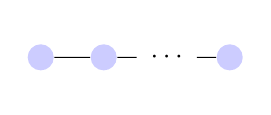
\begin{tikzpicture}
    [scale=.8,auto=left,every node/.style={circle,fill=blue!20}]
    \node (n1) at (1,1) {};
    \node (n2) at (2,1) {};
    \node[fill=white] (n3) at (3,1) {\(\cdots\)} ;
    \node (n4) at (4,1) {};
    \draw (n1) -- (n2) ;
    \draw (n2) -- (n3) ;
    \draw (n3) -- (n4) ;
  \end{tikzpicture}

 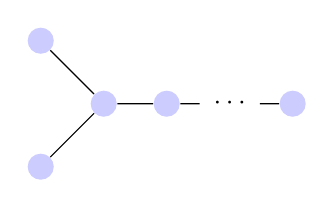
\begin{tikzpicture}
    [scale=.8,auto=left,every node/.style={circle,fill=blue!20}]
    \node (np) at (0,2) {};
    \node (nm) at (0,0) {};
    \node (n1) at (1,1) {};
    \node (n2) at (2,1) {};
    \node[fill=white] (n3) at (3,1) {\(\cdots\)};
    \node (n4) at (4,1) {};
    \draw (n1) -- (n2) ;
    \draw (n2) -- (n3) ;
    \draw (n3) -- (n4) ;
    \draw (nm) -- (n1) ;
    \draw (np) -- (n1) ;
  \end{tikzpicture}

  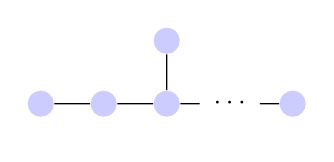
\begin{tikzpicture}
    [scale=.8,auto=left,every node/.style={circle,fill=blue!20}]
    \node (n1) at (1,1) {};
    \node (n2) at (2,1) {};
    \node (n3) at (3,1) {};
    \node (nu) at (3,2) {};
    \node[fill=white] (n4) at (4,1) {\(\cdots\)} ;
    \node (n5) at (5,1) {};
    \draw (n1) -- (n2) ;
    \draw (n2) -- (n3) ;
    \draw (n3) -- (n4) ;
    \draw (n4) -- (n5) ;
    \draw (n3) -- (nu) ;
  \end{tikzpicture}
  \caption{Dynkin graphs \(A_n\), \(D_n\), and \(E_{6,7,8}\)}
\end{figure}
\begin{figure}[h]
%  \centering
  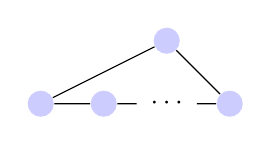
\begin{tikzpicture}
    [scale=.8,auto=left,every node/.style={circle,fill=blue!20}]
    \node (n1) at (1,1) {};
    \node (n2) at (2,1) {};
    \node[fill=white] (n3) at (3,1) {\(\cdots\)} ;
    \node (nu) at (3,2) {};
    \node (n4) at (4,1) {};
    \draw (n1) -- (n2) ;
    \draw (n2) -- (n3) ;
    \draw (n3) -- (n4) ;
    \draw (n1) -- (nu) ;
    \draw (n4) -- (nu) ;
  \end{tikzpicture}

 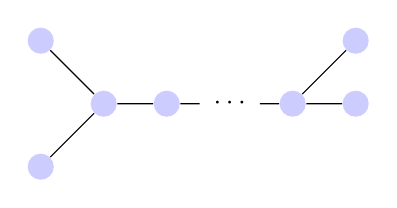
\begin{tikzpicture}
    [scale=.8,auto=left,every node/.style={circle,fill=blue!20}]
    \node (np) at (0,2) {};
    \node (nm) at (0,0) {};
    \node (n1) at (1,1) {};
    \node (n2) at (2,1) {};
    \node[fill=white] (n3) at (3,1) {\(\cdots\)};
    \node (n4) at (4,1) {};
    \node (n5) at (5,1) {};
    \node (n6) at (5,2) {};
    \draw (n1) -- (n2) ;
    \draw (n2) -- (n3) ;
    \draw (n3) -- (n4) ;
    \draw (nm) -- (n1) ;
    \draw (np) -- (n1) ;
    \draw (n4) -- (n5) ;
    \draw (n4) -- (n6) ;
  \end{tikzpicture}  
  \caption{Euclidean Dynkin graphs \(\hat{A}_n\) and \(\hat{D}_n\)}
  \label{fig:euclidean-dynkin}
\end{figure}
\begin{rmk}
  The difference from the ``Lie'' setting is here \(n_{ij} \in \Z\)
  where in the ``Lie'' setting, \(n_{ij} = \sqrt{a_{ij} a_{ji}}\). 
\end{rmk}
\begin{proof}[Proof of Theorem]
  The second part of the theorem is a ``boundary'' case. Any graph
  containing \(\widehat{ADE}\) has \(q_\Q\) indefinite and any graph
  not containing \(\widehat{ADE}\) is covered by the first case. 
\end{proof}
\begin{cor}
  Consider the ``star'' graph \(\Gamma(p,q,r)\) \\
  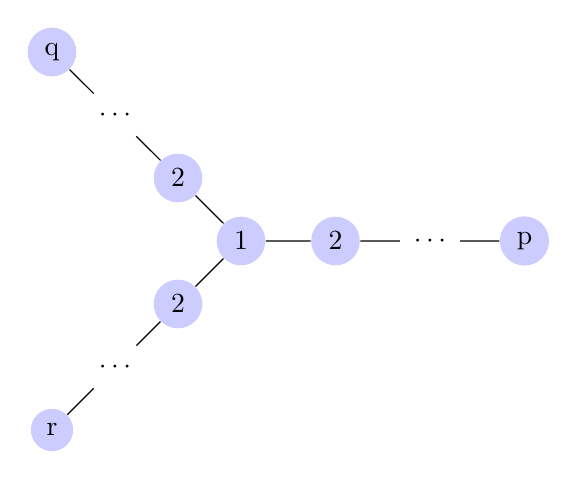
\begin{tikzpicture}
    [scale=.8,auto=left,every node/.style={circle,fill=blue!20}]
    \node (c) at (3,3) {1};
    \node (p2) at (4.5,3) {2} ;
    \node[fill=white] (p3) at (6,3) {\(\cdots\)} ;
    \node (pn) at (7.5,3) {p} ;
    \node (q2) at (2,4) {2} ;
    \node[fill=white] (q3) at (1,5) {\(\cdots\)} ;
    \node (qn) at (0,6) {q} ;
    \node (r2) at (2,2) {2} ;
    \node[fill=white] (r3) at (1,1) {\(\cdots\)} ;
    \node (rn) at (0,0) {r} ;
    \draw (c) -- (p2) ;
    \draw (c) -- (q2) ;
    \draw (c) -- (r2) ;
    \draw (p2) -- (p3) ;
    \draw (p3) -- (pn) ;
    \draw (q2) -- (q3) ;
    \draw (q3) -- (qn) ;
    \draw (r2) -- (r3) ;
    \draw (r3) -- (rn) ;
  \end{tikzpicture} \\
  Then, \(\Gamma(p,q,r)\) has positive-definite \(q_\Q\) if and only
  if \[
    \frac{1}{p} + \frac{1}{q} + \frac{1}{r} > 1
  \]
  which happens if and only if \((p,q,r)\) is of the following
  forms \[
    \begin{cases}
      (p,q,1) & A_{p+q-1} \\
      (p,2,2) & D_{p+2} \\
      (p,3,2) & p=3,4,5 \ \ E_{p+3}
    \end{cases}
  \]
\end{cor}
\todo{Understand why this is a corollary and why it is true.}
A natural question one may ask is about types \(B,C,F,G\). To do this,
we will have to do some more work. Due to the resemblence of these
constructions to Lie theory, we will use some similar definitions.
\begin{defn}
  Assume \(|\Q|\) has no edge loop, that is \(n_{ii} = 0\). Then, we
  define the \de{Cartan matrix} to be \[
    C_\Q := C_{|\Q|} = 2I-A
  \]
  where \(A = (n_{ij})\) is the adjacency matrix. 
\end{defn}
This matrix can be used to define Kac-Moody algebra \(\g = \g_\Q\) (or
simple Lie algebra if \(\Q\) is Dynkin). Then, we get the following.
\begin{defn}\label{root-lattice-dynkin-quiver}
  We define the \de{root latice} \(L = \bigoplus_{i \in I} \Z \alpha_i
  \isom \Z^I\) where \(\alpha_i = \grdim S(i)\) are the \de{simple
    roots}. This gives rise to \de{simple reflections} \(s_i \from L
  \to L\) defined by \(\alpha \mapsto \alpha - (\alpha,\alpha_i)
  \alpha_i\) and thus \de{Weyl group} \(W = \langle  s_i \st i \in I
  \rangle \subgroup GL(L \otimes_\Z \R\)
\end{defn}
\begin{prop}\label{dynkin-root-system-char}
  \begin{enumerate}
  \item \(W\) preserves \((\cdot, \cdot)\).
  \item For Dynkin (or Euclidean), the root system of \(\g\), \(R =
    \{\alpha \in L \setminus 0 \st (\alpha,\alpha) \leq 2\}\) (or
    \(=2\) if Dynkin). 
  \end{enumerate}
\end{prop}
Now, we are ready to discuss Gabriel's Theorem. We require \(\ov{\bbk}
= \bbk\).
\begin{defn}
  A quiver \(\Q\) is of \de{finite type} if the number of
  indecomposable representations of \(\Q\) of any fixed \(\grdim = 
  \vec{w}\) is finite.
\end{defn}
\begin{thm}[Gabriel's Theorem]\label{gabriels-thm}
  A connected quiver \(\Q\) is of finite type if and only if \(|\Q|\)
  is Dynkin (ie types \(ADE\)). Furthermore, if \(\Q\) is Dynkin then
  there is a one-to-one correspondance between indecomposables and
  positive roots in the root system \(R\). 
\end{thm}
\begin{proof}
  For the forward direction, assume \(\Q\) is of finite type. Then, for
  \(0 \neq \vec{v} \in \N^I\), there exists finitely many
  representations of \(\grdim = \vec{v}\). So, \(GL(\vec{v})\) acting
  on \(\Rep(\vec{v})\) has finitely many orbits. Therefore,
  \(\Rep(\vec{v}) = \ov{\O}_x\) for some \(x \neq 0\)
  \todo{why?}. Now, \(\dim \Rep(\vec{v}) = \dim \O_x = \dim
  GL(\vec{v}) - \dim G_x\) by \todo{why?}. Thus, we have \[
    1 \leq \dim G_x = \dim GL(\vec{v}) - \dim \Rep(\vec{v}) = q(\vec{v})
  \]
  since the identity matrix, \(I \in G_x \implies \dim G_x \geq 1
  \implies q(\vec{v}) \geq 1\). This completes the forward
  direction. We still must lay more groundwork to prove the rest of
  this theorem.
\end{proof}
\begin{prop}
  Given \(\vec{u} \in \Z^I\) and \(\vec{v}\) such that \(v_i = |u_i|\)
  for all \(i\), then \(q(\vec{v}) \leq q(\vec{u})\). 
\end{prop}
\begin{proof}
  \[
    q(\vec{v}) = \sum |u_i|^2 - \sum_h |u_{s(h)}| |u_{t(h)}| \leq \sum
    u_i^2 - \sum u_{s(h)} u_{t(h)} = q(\vec{u})
  \]
\end{proof}
\begin{example}
  Consider the quiver \[
    \begin{tikzcd}
      1 \rar & 2
    \end{tikzcd}
  \]
\end{example} \todo{finish this example}
\subsection*{(9/5/2017) Lecture 5}
\subsection{Reflection functors}
Starting off, this section is completely general and not restricted to
quivers of type \(ADE\).
\begin{defn}
  If a vertex \(i\) in a quiver \(\Q\) has no edges leaving \(i\), we
  call \(i\) a \de{sink}. \[ 
    \begin{tikzcd}
      \ar[rd]& & \\
      & i & \lar \\
      \ar[ru] & & 
    \end{tikzcd}
  \]
  Similarly, if a vertex \(i\) in a quiver \(\Q\) has no edges
  entering \(i\), we call \(i\) a \de{source}. \[
  \begin{tikzcd}
      \ & & \\
      & i \ar[r] \ar[lu] \ar[ld] & \  \\
      \ & & 
    \end{tikzcd}
  \]
\end{defn}
\begin{rmk}
  Note that \[
    \begin{tikzcd}
      \ar[r] & i \ar[r] & \
    \end{tikzcd}
  \]
  is neither a sink nor a source.
\end{rmk}
\begin{defn}
  We define reflections \(\sourcetosink_i\) and \(\sinktosource_i\) to flip
  all arrows incident to \(i\) and are defined as
  follows \[
    \begin{tikzcd}
      \text{source} \ar[r, bend left, "\sourcetosink_i"] & \ar[l, bend
      left, swap, "\sinktosource_i"] \text{sink}
    \end{tikzcd}
  \]
\end{defn}
\begin{prop}
  \(\sinktosource_i \sourcetosink_i (\Q) = \Q\)  for \(i\) a sink in \(\Q\).
\end{prop}
\todo{Prove this or at least do a basic example.}
\begin{prop}
  Assume \(|\Q|\) is a tree. Let \(\Omega, \Omega'\) be 2
  orientations of \(|\Q|\). Then, \(\Q'\) is obtained from \(\Q\) via
  a sequence of \(\sinktosource_i\) and \(\sourcetosink_i\) operations.
\end{prop}
\begin{proof}
  The proof proceeds by indcution on the number of vertices. Locate a
  sink or a source with one incident edge, which must exist since
  \(|\Q|\) is a tree. Call it 
  \(k\). Then,
  by the inductive hypothesis, one can obtain the orientation on the
  other vertices consistent wiht \(\Q'\). At this point, either the
  edge incident to \(k\) is in the correct orientation or it is
  not. If not, apply \(s_k\) and you are done.
\end{proof}
\begin{defn}
  For a sink \(i\) of \(\Q\), let \(\Q' =
  \sinktosource_i(\Q)\). Define \[
    \sinktosourcefunc_i \from \Rep(\Q) \to \Rep(\Q')
  \]
  and take \(V \in \Rep(\Q)\). Then, if \(V' = \sinktosourcefunc_i(V)\),
  we have that \(V_j' = V_j\) when \(j \neq i\) and \[
    V_i' = \sinktosourcefunc_i(V)_i = \ker\left( \bigoplus_{k \to i}
      V_k \to V_i \right)
  \]
  Thus, \(\sinktosourcefunc_i\) only changes the vector space at \(i\)
  and the maps to and from \(i\). 
\end{defn}
\begin{defn}
  For source \(i\) at \(\Q\), let \(\Q' =
  \sourcetosink_i(\Q)\). Similar to the above, we can define \[
    \sourcetosinkfunc_i \from \Rep(\Q) \to \Rep(\Q')
  \]
  where \(\sourcetosinkfunc_i(V)_i = \coker \left( V_i \to \bigoplus_{i
      \to k} V_k \right)\)
\end{defn}
\begin{rmk}
  These functors are called the \de{BGP reflection functors}.
\end{rmk}
\begin{example}
  We note that \(\sinktosourcefunc_i(S(i)) =
  0\) where \(i\) is a sink in \(\Q\). This happens because \(\ker
  \left( \bigoplus_{k \to i} V_k \to 
    V_i \right)\) but, \(\bigoplus_{k \to i} V_k = 0\). Similarly
  \(\sourcetosinkfunc_i(S(i)) = 0\) since \(V_i \to \bigoplus_{i \to
    k} V_k = 0\) so the codomain is trivial and thus \(\coker(V_i \to
  \bigoplus_{i \to k} V_k)\). 
\end{example}
\begin{example}
  Let \(\Q\) be the quiver \[
    \begin{tikzcd}
      1 \rar & 2
    \end{tikzcd}
  \]
  and consider the representation \[
    V = \begin{tikzcd}
      \bbk \rar & 0
    \end{tikzcd}
  \]
  Then, \(\sinktosourcefunc_2(V)_2 = \ker \left( \bigoplus_{k \to 2}
    V_k \to V_2 \right) = \ker \left( V_1 \to V_2 \right) = \ker(\bbk
  \to 0)\). So, we get \[
    V' := \sinktosourcefunc_2(V) =
    \begin{tikzcd}
      \bbk & \lar \bbk
    \end{tikzcd}
  \]
  Now, if we apply \(\sourcetosinkfunc_2(V')\), we see that we get
  \(\coker \left( \bbk \to \bbk \right) = 0\), so we actually recover
  \(V\). Now, take \(\sourcetosinkfunc_1(V')\). Since \(\ker \left(
    \bigoplus_{k \to 1} V_k \to V_1 \right) = \ker \left( \bbk \to
    \bbk \right) = 0\). So, \[
    W := \sinktosourcefunc_2(V') =
    \begin{tikzcd}
      0 \rar & \bbk
    \end{tikzcd}
  \]
  Similarly, \(\sourcetosinkfunc_1(W) = V'\) since we are taking
  \(\coker ( 0 \to \bbk) \isom \bbk\). Now, notice that these are the
  3 indecomposables and the correspond to the 3 positve roots (2
  simple). To see this, note that \(|\Q|\) is of type \(A_2\), so it
  has 2 simple roots \(\beta = (0,1)\) and \(\alpha = (1,0)\). Then, we get the
  correspondance using graded dimension
  
  \[
    \begin{tikzcd}
      (\bbk \rar & 0)  \ar[r, mapsto] & (1,0) \text{ is simple}\\
      (\bbk & \lar \bbk) \ar[r, mapsto] & (1,1)\\
      (0 \rar & \bbk) \ar[r,mapsto] & (0,1) \text{ is simple}
    \end{tikzcd}
\]  
\end{example}
\begin{example}\label{ex-a3}
  Take the quiver \(\Q\) and \(V\), a representation, to be \[
    \begin{tikzcd}
      1 \rar & 2 & \lar 3
    \end{tikzcd}, \ \ \
    \begin{tikzcd}
      0 \rar & 0 & \lar \bbk
    \end{tikzcd}
  \]
  Then, we can apply \(\sinktosourcefunc_2\) to \(V\) to get
  \(V'\). We compute that \[
    V'_2 = \ker\left(\bigoplus_{k \to 2} V_k \to V_2\right) = \ker(\bbk \to 0) = \bbk
  \]
  So, \[
    V' =
    \begin{tikzcd}
      0 & \lar \bbk \rar & \bbk
    \end{tikzcd}
  \]
  Doing similar computations, we get the following diagram \[
    \begin{tikzcd}
      & & 0 & \lar \bbk \rar \ar[dll, dashed, "\sinktosourcefunc_1"]
      \ar[drr, dashed, "\sinktosourcefunc_3"]& \bbk & & \\
      \bbk \rar & \bbk \rar \ar[drr, dashed, "\sinktosourcefunc_3"] &
      \bbk & & \bbk & \lar \bbk \ar[dll, dashed, "\sinktosourcefunc_1"] & \lar 0 \\
      & & \bbk \rar & \bbk \ar[d, dashed, "\sinktosourcefunc_2"] & \lar 0 & & \\
      & & \bbk & \lar 0 \rar & 0
    \end{tikzcd}
  \]
\end{example}
\begin{example}\label{refl-func-non-inverse-ex}
  Let \(\Q\) be a quiver and \(V\), a representation of \(\Q\), given
  by \[
    \begin{tikzcd}
      1 \rar & 2 & \lar 3
    \end{tikzcd} \ \ \
    \begin{tikzcd}
      0 \rar & \bbk & \lar 0
    \end{tikzcd}
  \]
  If we apply \(\sourcetosinkfunc_1(V) =: V'\), we see that \[
    V'_1 = \coker\left( V_1 \to \bigoplus_{1 \to k} V_k \right) =
    \coker(0 \to \bbk) = \bbk
  \]
  So, we get the following \[
    \sourcetosinkfunc_1(V) =
    \begin{tikzcd}
      \bbk & \lar \bbk & \lar 0
    \end{tikzcd} \ \ \ 
    \sourcetosinkfunc_3(V) =
    \begin{tikzcd}
      0 \rar & \bbk \rar & \bbk
    \end{tikzcd}
  \]
  where the second equality follows from symmetry. However, note that
  \[
    \sinktosourcefunc_2(V)_2 = \ker\left( \bigoplus_{k \to 2} V_k \to
      V_2 \right) = \ker(0 \to \bbk) = 0 \implies
    \sinktosourcefunc_2(V) =
    \begin{tikzcd}
      0 & \lar 0 \rar & 0
    \end{tikzcd}
  \]
  Thus, we have found a situation where \(\sinktosourcefunc_i\) and
  \(\sourcetosinkfunc_i\) are not inverses! \todo{Finish these
    computations.} 
\end{example}
\begin{prop}\label{right-derived-func-is-0}
  For sink \(i\) of \(\Q\), \(\sinktosource_i\) is left
  exact. Furthermore, the right derived functor \(R^n \sinktosourcefunc_i
  = 0\) for \(n > 1\). Finally, \[
    R^1 \sinktosourcefunc_i(V) = 0 \iff \bigoplus_{k \to i} V_k \to V_i
    \text{ is surjective. Call this property }\left(\overset{\downarrow}{i}\right)
  \]
\end{prop}
\begin{defn}
  In the case of the above proposition, we define \(\Rep^{i
    \leftarrow}\) is the full subcategory of \(\Rep(\Q)\) consisting
  of objects \(V\) that satisfy \(\left( \overset{\downarrow}{i} \right)\).
\end{defn}
\begin{prop}
  For source \(i\) of \(\Q\), \(\sourcetosinkfunc_i\) is right
  exact. Furthermore, the left derived functor \(L^n
  \sourcetosinkfunc_i = 0\) for \(n > 1\). Finally, \[
    L^1 \sourcetosinkfunc_i (V) = 0 \iff V_i \to \bigoplus_{i \to k}
    V_k \text{ is injective. Call this property } \left(
      \overset{\uparrow}{i} \right).
  \]
\end{prop}
\begin{defn}
  In the case of the above proposition, we define \(\Rep^{i
    \rightarrow}\) is the full subcategory of \(\Rep(\Q)\) consisting
  of objects \(V\) that satisfy \(\left( \overset{\uparrow}{i} \right)\).
\end{defn}
\begin{rmk}
  We will end up showing that \(\Rep^{i \leftarrow}(\Q)\) and
  \(\Rep^{i \rightarrow}(\Q)\) contain all indecomposables of \(\Q\)
  except for \(S(i)\). In a sense, this encodes the same fact that a
  reflection \(s_i\) on a positive set of roots \(\roots_+\) takes the set
  \(\roots_+ \setminus \{\alpha_i\}\) to \(\roots_+ \setminus
  \{\alpha_i\}\). This becomes explicitly manifest in
  \ref{indec-are-positive}. \todo{I understand this, but get a much better
    handle on it. And what is this reference?}
\end{rmk}
\begin{proof}[Proof of Above Propositions]
  \todo{Understand this proof...}
\end{proof}
\begin{prop} \label{source-sink-adjointness}
  For \(i\) a sink of \(\Q\), let \(\Q' = \sinktosource(\Q)\). Then,
  \(\sinktosourcefunc_i\) and \(\sourcetosinkfunc_i\) are an adjoint
  pair. That is, for \(W \in \Rep(\Q)\) and \(V' \in \Rep(\Q')\), we
  get \[
    \Hom_\Q(\sourcetosinkfunc_i(V'), W) \isom \Hom_{\Q'}(V',
    \sinktosourcefunc_i(W)) 
  \]
\end{prop}
\begin{proof}
  Consider that the cokernel is the universal object such that the
  following diagram commutes \[
    \begin{tikzcd}
      \bigoplus_{i \to k} V_k' \ar[dr]& \\
      V_i' \ar[u] \ar[r, "0"]& \coker(V_i' \to \bigoplus_{i \to k} V_k)
    \end{tikzcd}
  \]
  Similarly, the kernel is the universal object such that the
  following diagram commutes \[
    \begin{tikzcd}
      \bigoplus_{k \to i} W_k \ar[dr]& \\
      \ker(\bigoplus_{k \to i} W_k \to W_i) \ar[u] \ar[r,"0"]  & W_i 
    \end{tikzcd}
  \]
  So, let \(f \in \Hom_Q(\sourcetosinkfunc_i(V'),W)\) map
  \(\coker(V_i' \to \bigoplus_{i \to k} V_k) \to W_i\). Then, we
  get \[
    \begin{tikzcd}
      & &  \bigoplus_{k} W_k \ar[d,"pr"]\\
      \bigoplus_{i \to k} V_k' \ar[rru, bend left, "\bigoplus_{i \to k} f_k"]& \ker(\bigoplus_k W_k \to W_i)
      \ar[r,"0"] \ar[ru]& W_i \\
      V_i' \ar[u] \ar[r, color=gray, "0"] \ar[rru, bend right=40, "0"] \ar[ru,
      dashed, "\exists\unique"]& \coker(V_i' \to \bigoplus_{i \to k}
      V_k) \ar[ru, color=gray, "f_i"] & 
    \end{tikzcd}
  \]
  Thus, a map \(f \in \Hom_Q(\sourcetosinkfunc_i(V'),W)\) induces a
  unique map in \(\Hom_{Q'}(V',
  \sinktosourcefunc_i(W))\). Similarly, given a \(g \in
  \Hom_{Q'}(V', \sinktosourcefunc_i(W))\), we get \[
  \begin{tikzcd}
      \bigoplus_{i \to k} V_k' \ar[dr] \ar[drr, bend left,
      "\bigoplus_k g_k"]& \\
      V_i' \ar[u] \ar[r, "0"] \ar[dr, "g_i", color=gray] \ar[drr, bend right=40, "0"]& \coker(V_i' \to \bigoplus_{i \to k}
      V_k) \ar[rd, dashed, "\exists\unique"] & \bigoplus_k W_k \ar[d] \\
      &  \ker(\bigoplus_{k} W_k \to W_i) \ar[r, color=gray, "0"]& W_i
    \end{tikzcd}
  \]
  So, a map \(g \in \Hom_{Q'}(V', \sinktosourcefunc_i(W))\)
  corresponds to a unique map in
  \(\Hom_Q(\sourcetosinkfunc_i(V'),W)\). Therefore,
  \(\sourcetosinkfunc_i\) and \(\sinktosourcefunc_i\) form an adjoint
  pair. 
\end{proof}
\begin{prop}
  With the same situation as above, \(\sinktosourcefunc_i(W) \in \Rep^{i
    \rightarrow}(\Q')\) and \(\sourcetosinkfunc_i(V') \in \Rep^{i
    \leftarrow}(\Q)\).
\end{prop}
\begin{proof}
  By definition, \(\Rep^{i \rightarrow}(Q')\) is all representations
  that have \(V_i \into \bigoplus_{i \to k} V_k\). However,
  \(\sinktosourcefunc_i(W)_i = \ker(\bigoplus_{k \to i}W_k \to W_i)
  \into \bigoplus_{i \to k} W_k\), by definition. Note that the
  reflection functor changes all edges that were \(k \to i\) into \(i
  \to k\) edges. \\

  Similarly, \(\Rep^{i \leftarrow}(Q)\) is all
  representations that have \(\bigoplus_{k \to i} V_k \onto V_i\) and
  \(\sourcetosinkfunc_i(V')_i = \coker(V'_i \to \bigoplus_{k \to i}
  V_k) \onto V'_i\) by definition, and since \(\bigoplus_{i \to k} V'_k
  \onto \coker(V'_i \to \bigoplus_{k \to i} V'_k) \onto V'_i\), we are
  done.
\end{proof}
\begin{prop}\label{equiv-of-cats-source-sink}
  As functors, \(\sourcetosinkfunc_i\) and \(\sinktosourcefunc_i\) are
  inverses between \(\Rep^{i \rightarrow}(\Q)\) and \(\Rep^{i
    \leftarrow} \Q\)
\end{prop}
\begin{proof}
  We want to show that \(\sourcetosinkfunc_i \sinktosourcefunc_i (W) \isom W\)
  for \(W \in \Rep^{i \leftarrow}(\Q)\). Now, since \(W \in \Rep^{i
    \leftarrow}(\Q)\), then, by definition, we get \[
    \bigoplus_{k \to i} W_k \onto W_i
  \]
  Thus, it must be that
  \begin{align*}
    \sourcetosinkfunc_i(\sinktosourcefunc_i(W))_i
    & = \coker\left(\ker \left( \bigoplus_{k \to i} W_k \onto W_i
      \right) \to \bigoplus_k W_k\right) \\ 
    & = \left(\bigoplus_k W_k\right) / \ker \left( \bigoplus_{k \to i}
      W_k \onto W_i \right) \\
    & = \im \bigoplus_{k \to i} W_k \onto W_i \\
    & = W_i
  \end{align*}
\end{proof}
\begin{prop}\label{relate-refl-to-refl-func}
  Let \(\Q\) be arbitrary quiver. Let \(s_i = s_{\alpha_i} \from \Z^I
  \to \Z^I\) be the simple 
  reflection sending \(\alpha \mapsto \alpha - (\alpha, \alpha_i)
  \alpha_i\), see \ref{root-lattice-dynkin-quiver}. 
  \begin{enumerate}
  \item For \(W \in \Rep^{i \leftarrow}(\Q)\), \[
      \grdim \sinktosourcefunc_i(W) = s_i(\grdim W)
    \]
  \item For \(V' \in \Rep^{i \rightarrow}(\Q)\), \[
      \grdim \sourcetosinkfunc_i(V') = s_i(\grdim V')
    \]
  \end{enumerate}
\end{prop}
\begin{proof}
  For the first part, we know that \(W\) has the property that
  \(\bigoplus_{k \to i} W_k \onto W_i\) so \(\dim
  (\sinktosourcefunc_i(W))_i = \sum_{k \to i} (\dim W_k) - \dim W_i\). First,
  we compute that, if \(j\) is not incident to \(i\), then \(s_i(\alpha_j) =
  \alpha_j\), if \(k \to i\), then \[
    (\alpha_k, \alpha_i) = \left(\sum_{j \in I} (\alpha_k)_j (\alpha_i)_j -
    \sum_{h \in \Omega} (\alpha_k)_{s(h)} (\alpha_i)_{t(h)} \right) +
  \left(
    \sum_{j \in I} (\alpha_i)_j (\alpha_k)_j -
    \sum_{h \in \Omega} (\alpha_i)_{s(h)} (\alpha_k)_{t(h)}
  \right)    
\]
However, since \((\alpha_i)_j = \delta_{ij}\), \((\alpha_k)_j =
\delta_{kj}\), and \(i \neq k\), then the vertex indexed sums will be
0. Furthermore, there is only one edge \(k \to i\), so the first sum
will be \(1\) and the other will be \(0\). Thus, we get \[
  (\alpha_k, \alpha_i) = -1 \implies s_i(\alpha_k) = \alpha_k -
  (\alpha_k, \alpha_i) \alpha_i = \alpha_k + \alpha_i
\]
We also compute that \[
  (\alpha_i, \alpha_i) = 2 \sum_{j \in I} (\alpha_i)_j^2 - 2 \sum_{h
    \in \Omega} (\alpha_i)_{s(h)} (\alpha_i)_{t(h)} = 2
\]
  and so \(s_i(\alpha_i) = \alpha_i - (\alpha_i,\alpha_i) \alpha_i =
  -\alpha_i\). 
  Now, we compute that
  \begin{align*}
    s_i(\grdim W)
    & = s_i \left( \sum_{j \text{ not incident to }i} w_j
      \alpha_j  + \sum_{k \to i}(w_k \alpha_k) + w_i \alpha_i 
      \right)  \\
    & = \sum_{j \text{ not incident to }i} w_j \alpha_j + \sum_{k \to i}( w_k (\alpha_k + \alpha_i)) - w_i \alpha_i \\
    & = \sum_{j \neq i} w_j \alpha_j + \sum_{k \to i}( w_k \alpha_i )
      - w_i \alpha_i \\
    & = \grdim \sinktosourcefunc_i(W)
  \end{align*}
  A similar computation works for part (b).
\end{proof}
\begin{rmk}
  Let \(\derivcat(\Q) := \derivcat(\Rep(\Q))\). Then, \(\derivcat(\Q)
  \isom \derivcat(\Q')\).\todo{Cite lecture notes by Milicic.} \todo{Always? Or \(Q,Q'\) as above?}
\end{rmk}
\subsection*{(9/7/2017) Lecture 6}
\begin{prop}
  Let \(\Q\) be a quiver.
  \begin{enumerate}
  \item For \(i\) a sink for \(\Q\) and \(\Q' = \sinktosource_i \Q\),
     if \(V \in \Rep^{i
      \leftarrow}(\Q)\), \(W \in \Rep(\Q)\), then \[
      \Hom_\Q(V,W) \isom \Hom_{\Q'}(\sinktosourcefunc_i V,
      \sinktosourcefunc_i W)
    \]
  \item For \(i\) a source for \(\Q\), if \(V \in \Rep(\Q), W \in
    \Rep^{i \rightarrow}(\Q)\), then \[
      \Hom_\Q(V,W) \isom \Hom_{\Q'}(\sourcetosinkfunc_i V,
      \sourcetosinkfunc_i W)
    \]
  \end{enumerate}
\end{prop}
\begin{proof}
  For part (a), consider that \(V =
  \sourcetosinkfunc_i(\sinktosourcefunc_i V)\) by
  \ref{equiv-of-cats-source-sink}, then we can apply the adjointness 
  (\ref{source-sink-adjointness}) to get \[
    \Hom_\Q(\sourcetosinkfunc_i(\sinktosourcefunc_i V), W) \isom
    \Hom_{\Q'}(\sinktosourcefunc_i V, \sinktosourcefunc_i W)
  \]
  A dual argument applies for part (b).
\end{proof}
\begin{defn}\label{choice-of-positive}
  Let \(\vec{v} \in \Z^{\geq 0}\). Then, we say \((v_i)_{i \in I} =
  \vec{v} > 0 \iff v_i \geq 0\) for all \(i \in I\).
\end{defn}
\begin{prop}\label{indec-are-pos}
  Let \(0 \neq V \in \Rep(\Q)\) be indecomposable, \(i\) a sink/source. Then,
  \begin{enumerate}
  \item If \(V \isom S(i)\), then \(\sinksourcefunc_i(V) = 0\).
  \item If \(V \not\isom S(i)\), then \(V \in \Rep^{i
      \substack{\leftarrow \\ \rightarrow}}(\Q)\).
  \item \(\sinksourcefunc_i(V)\) is nontrivial and indecomposable if
    and only if \(s_i(\grdim V) \geq 0\).
  \end{enumerate}
\end{prop}
\begin{proof}
  Part (a) follows from computations like in example
  \ref{refl-func-non-inverse-ex}. For part (b), if \(V \not \in
  \Rep^{i \leftarrow}(\Q)\), then \(\bigoplus_{k \to i} V_k \overset{f}{\to}
  V_i\) is \emph{not} surjective. So, we can take \(V_i = \im(f)
  \oplus V_i''\) with \(V_i'' \neq 0\). Define \(V',V'' \in
  \Rep(\Q)\) by \[
    V_j' =
    \begin{cases}
      V_j & j \neq i \\
      \im(f) & j = i
    \end{cases}, \ \ 
    V_j'' =
    \begin{cases}
      0 & j \neq i \\
      V_i'' & j = i
    \end{cases}
  \]
  Then, \(V = V' \oplus V''\), which contradicts the indecomposability
  of \(V\). To show that nontrivial, indecomposable \(V \in \Rep^{i
    \rightarrow}\) for \(i\) a source, assume, as above, that
\(\bigoplus_{k \to i} V_k \overset{f}{\to} 
  V_i\) is not surjective. \todo{Finish this part of the proof. Maybe
    ask for a hint!} \\

  For part (c), the proof follows from (a), (b), and
  \ref{relate-refl-to-refl-func}. \todo{Write the actual proof. I do
    not see quite how to connect these facts to get what we want. Help!}
\end{proof}
\begin{prop}
  Let \(\Q\) be a quiver and \(\Q' = \sinksource \Q\). 
  \begin{enumerate}
  \item For sink \(i\) of \(\Q\), if \(V \in \Rep(\Q), W \in \Rep^{i
      \leftarrow}(\Q)\), then \[
      \Ext_\Q^1(V,W) \isom \Ext_{Q'}^1(\sinktosourcefunc_i V,
      \sinktosourcefunc_i W).
    \]
  \item For source \(i\) of \(\Q\), if \(V \in \Rep^{i
      \rightarrow}(\Q), W \in \Rep(\Q)\), then \[
      \Ext_\Q^1(V,W) = \Ext_{\Q'}^1(\sourcetosinkfunc_i V,
      \sourcetosinkfunc_i W).
    \]
  \end{enumerate}
\end{prop}
\begin{example}
  One could have assumed \(V,W \in \Rep^{i \leftarrow}\) to get more
  restrictive theorems, but we can check that \(S(i)\), which is not
  in \(\Rep^{i \leftarrow}\), will work if put in the right
  spots. Namely,
  \begin{align*}
    \Hom_\Q(V,S(i)) = 0 \\
    \Ext_\Q(S(i),W) = 0
  \end{align*}
  where the second equality follows because \(S(i) = P(i)\) when \(i\)
  is a sink. Thus, we have found a useful way to remember that we can
  enlarge the possible category for \(W\) in the \(\Hom\) case and
  enlarge the possible category of \(V\) in the \(\Ext\) case.
\end{example}
\begin{proof}[Proof of Proposition]
  For part (a), if \(V \isom S(i)\), we just showed in the above
  example that the left side is trivial and the right side is trivial
  using part (a) of 
  \ref{indec-are-pos}. Furthermore, by general homological algebra, we
  know that \[ 
    \Ext_\Q^1(\bigoplus_{\alpha} V_\alpha, W) \isom \prod_{\alpha}
    \Ext_\Q^1(V_\alpha, W)
  \]
  and so it suffices to consider \(V\) as indecomposable. By part (b)
  of \ref{indec-are-pos}, since \(V \not \isom S(i)\), then \(V \in
  \Rep^{i \leftarrow}(\Q)\). Now, consider the short exact sequence in
  \(\Rep(\Q)\) given by \[
    0 \to W \to M \to V \to 0
  \]
  representing an element in \(\Ext_\Q^1(V,W)\). Using the right
  derived functor \(R\sinktosourcefunc_i\), we get long exact
  sequence \[
    0 \to \sinktosourcefunc_i W \to \sinktosourcefunc_i M \to
    \sinktosourcefunc_i V \to R^1 \sinktosourcefunc_i W \to
    R^1 \sinktosourcefunc_i M \to R^1 \sinktosourcefunc_i V \to 0
  \]
  However, \(R^1 \sinktosourcefunc_i V = 0 = R^1 \sinktosourcefunc_i
  W\) since \(V,W \in \Rep^{i
      \leftarrow}(\Q)\) (\ref{right-derived-func-is-0}). So, this forces
    \(R^1 \sinktosourcefunc_i M = 0 
  \implies M \in \Rep^{i \leftarrow}(\Q)\). Furthermore, we are left
  with the short exact sequence \[
    0 \to \sinktosourcefunc_i W \to \sinktosourcefunc_i M \to
    \sinktosourcefunc_i V \to 0
  \]
  which represents an element in \(\Ext_\Q^1(\sinktosourcefunc_i V,
  \sinktosourcefunc_i W)\). Thus, we have a map \(\Ext_\Q^1(V,W) \to
  \Ext_{\Q'}(\sinktosourcefunc_i V, \sinktosourcefunc_i W)\). We can
  then make a similar argument with \(\Ext_{\Q'}^i(\sinktosourcefunc_i
  V, \sinktosourcefunc_i W) \to \Ext_{\Q}^1(\sourcetosinkfunc_i \sinktosourcefunc_i
  V, \sourcetosinkfunc_i \sinktosourcefunc_i W) =
  \Ext_Q^1(V,W)\). These two maps are inverse to each other
  \todo{Actually check this?}
\end{proof}
\begin{prop}
  Assume \(i\) is a sink (or source) of \(\Q\) and \(\Q' = \sinksource
  \Q\). If, for \(a=1,2\), \(0 \neq I_a \in
  \Rep(\Q)\) is indecomposable and \(\sinksourcefunc_i(I_a) \neq 0\) (thus
  indecomposable), then
  \begin{align*}
    \Hom_\Q(I_1,I_2) \isom \Hom_{\Q'}(\sinksourcefunc_i I_1,
    \sinksourcefunc_i I_2) \\
    \Ext_\Q^1(I_1, I_2) \isom \Ext_{\Q'}^1(\sinksourcefunc_i I_1,
    \sinksourcefunc_i I_2)
  \end{align*}
\end{prop}
We now return back to the program of proving Gabriel's theorem
(\ref{gabriels-thm}).
\begin{rmk}
  For all quivers \(\Q\) without edge loops, there exists a
  correspondance between the indecomposable representations of \(\Q\)
  and the positive roots of its root system. In fact, the real
  positive roots have a one-to-one correspondance, but the imaginary
  roots correspond to ``a family'' of indecomposables. Counting these
  families gives rise to the Kac polynomials \(K_\alpha(q) = a_0 q^N +
  \cdots + a_N\) where \(N\) is the dimension of the ``family'',
  \(a_N\) is the multiplicity of \(\alpha\) as a root, and \(a_i \in
  \N\). This is due to a conjecture by Kac that has been subsequently proven.
\end{rmk}
\begin{lem}\label{lemma-star}
  Assume \(\Q\) is a Dynkin quiver and \(0 \neq \vec{v} \in
  \Z^{|I|}_{\geq 0}\). Then, there exists a sequence \(i_1, \ldots,
  i_{k+1} \in I\) such that
  \begin{align*}
    i_1 \text{ is a sink for } & \Q \\
    i_2 \text{ is a sink for } & \sinktosource_{i_1}(\Q) \\
    i_3 \text{ is a sink for } & \sinktosource_{i_2}
                                 \sinktosource_{i_1}(\Q) \\
    \vdots & \\
    i_{k+1} \text{ is a sink for } & \sinktosource_{i_k} \cdots
                                     \sinktosource_{i_1}(\Q) 
  \end{align*}
  and \(\vec{v} \geq 0, s_{i_1}(\vec{v}) \geq 0, \ldots, s_{i_k}
  \cdots s_{i_1}(\vec{v}) \geq 0\), but \(s_{i_{k+1}} s_{i_k} \cdots
  s_{i_1}(\vec{v}) \not \geq 0\).
\end{lem}
\begin{defn}\label{defn-adapted}
  We say a sequence \(i_1, \ldots, i_{k+1} \in I\) meeting only the
  sink conditions (not necessarily the positivity ones), is
  \de{adapted} to an orientation \(\Omega\) of \(\Q\) with no oriented
  cycles. 
\end{defn}
Now, with this lemma in hand (whose proof we will postpone), we seek
to prove the second part of Gabriel's theorem.
\begin{proof}[Proof of Gabriel's Theorem (continued)]
  Given any indecomposable \(V \neq 0\) and \(\vec{v} = \grdim V\), we
  can construct a sequence \(i_1, \ldots, i_{k+1} \in I\) that is
  adapted to \(\Omega\). Then,
  \begin{align*}
    \sinktosourcefunc_{i_1}(V) \neq 0 \\
    \sinktosourcefunc_{i_2}\sinktosourcefunc_{i_1}(V) \neq 0 \\
    \vdots\\
    V' := \sinktosourcefunc_{i_k} \cdots \sinktosourcefunc_{i_1}(V) \neq 0
  \end{align*}
  and \(\sinktosourcefunc_{i_{k+1}}(V') = 0\). Thus, it must be that
  \(V' = S(i_{k+1})\) and so, we can work backwards to get \(V =
  \sourcetosinkfunc_{i_1} \cdots \sourcetosinkfunc_{i_k}(S(i_{k+1}))\)
  and thus, by \ref{relate-refl-to-refl-func}, \[
    \grdim V = s_{i_1} \cdots s_{i_k}(\alpha_{i_{k+1}}) \in \roots_+
  \]
  where the root is positive the lemma above. So, we have \[
    \Ext^1(V,V) = \cdots = \Ext^1(S(i),S(i)) = 0
  \]
  since \(S(i) = P(i)\), and so, by \ref{dim-of-ext-vv}, \(\O_V\) is open
  in \(\Rep(\vec{v})\). 
\end{proof}
Thus, our proof is complete modulo proving the lemma, which will be
our program for the next lecture.
\subsection*{(9/12/2017) Lecture 7}
For a quiver \(\Q\), recall that we can take \(L := \Z^I\) to be a
root lattice and take a set of simple roots \(\{\alpha_i \st i \in
I\}\) and then get a Weyl group \(W = \langle s_i \rangle_{i \in
  I}\) that acts on the roots. Using this Weyl group, we can define a
total order on \(I = \{i_1, \ldots, i_r\}\).
\begin{defn}
  Let \(C := s_{i_r} \cdots s_{i_1} \in W\). \(C\) is a \de{Coxeter
    element of \(W\)}. A Coxeter element depends on a choice of simple
  roots and the ordering of the simple roots. 
\end{defn}
\begin{example}
  Take \(W = S_n\) and simple reflections given by \(\{(i, i+1)\}_{i
    \leq n-1}\). Then a Coxeter element is \((1, 2, \ldots, n)\). So,
  if \(n=4\), then there are \(6\) \(4\)-cycles, which are all
  Coexeter elements.
\end{example}
\begin{prop}
  All Coxeter elements are \(W\)-conjugate.
\end{prop}
\begin{proof}
  (Lifted from Humphrey's ``Reflection Groups and Coxeter Groups''
  74--75).  From basic Lie algebras, we know that all simple systems are
  \(W\)-conjugate. So, it suffices to show that, for a fixed set of
  simples, the Coxeter elements resulting from different orderings of
  the roots are conjugate. Any cyclic permutation of indices will give
  a conjugate element \[
    s_n s_1 \cdots s_{n-1} = s_n (s_1 \cdots s_n) s_n
  \]
  Also, an interchange of an adjacent commuting pair of \(s_i, s_j\)
  will not change the Coxeter element. Using an inductive argument,
  one can show that all permutations of the indices can be acheived
  using combinations of these two types of permutations.
\end{proof}
\begin{defn}
  We define \(|C| = h\) (the order of \(C\) in \(W\)) to be the
  \de{Coxeter number}. 
\end{defn}
\begin{example}
  When \(W = S_n\), we can take \(s_i = (i, i+1)\) and thus \(C =
  (1,2, \ldots, n)\) and so the Coxeter number is just \(n\). When \(W
  = D_{2m}\), then \(C\) is a product of two generating reflections,
  and thus a rotation by \(\frac{2 k \pi}{m}\) where \(k\) is relatively
  prime to \(m\), and so it has order \(m\), which is thus the Coxeter
  number. 
\end{example}
\begin{prop} \label{coxeter-fixes-only-rad}
  Let \(x \in L_\R = \R \otimes_\Z L\). Then, \(Cx = x\) if and only if
  \(x \in \Rad(\cdot, \cdot)\), the radical of the form \((\cdot, \cdot)\).
\end{prop}
\begin{proof}
  Let \(Cx = x\). Then,
  \begin{align*}
    s_{i_r} \cdots s_{i_1} x = x
    & \implies s_{i_{r-1}} \cdots s_{i_1}x = s_{i_r} x \\
    & \implies s_{i_{r-1}} \cdots s_{i_1}x - x = s_{i_r} x - x = x -
      (x, \alpha_{i_r})\alpha_{i_r} - x = (x, \alpha_{i_r})\alpha_{i_r}
  \end{align*}
  However, the right hand side must be a multiple of \(\alpha_{i_r}\)
  and the left hand side must be a linear combination of
  \(\{\alpha_{i_1}, \ldots, \alpha_{i_{r-1}}\}\), so the only way this
  can happen is if both sides are \(0\). Thus, \((x, \alpha_{i_r}) =
  0\). Now, once can repeat this process to get \[
    s_{i_{r-1}} \cdots s_{i_1} x = x \implies \cdots \implies
    \begin{cases}
      (x, \alpha_{i_{r-1}}) = 0 \\
      \vdots \\
      (x, \alpha_{i_1}) = 0
    \end{cases}
  \]
  and thus \(x \in \Rad(\cdot, \cdot)\). \\

  If \(x \in \Rad(\cdot, \cdot)\), then \(s_i(x) = x -
  (x,\alpha_i)\alpha_i = x\) by definition, so \(C x = s_{i_{r}}
  \cdots s_{i_1} x = x\). 
\end{proof}
\begin{example}
  One non-trivial example is with quivers of type
  \(\widehat{ADE}\). There is only one imaginary root, \(\delta\) and
  \(s_i(\delta_i) = \delta_i\) for all \(i\).
\end{example}
\begin{prop}
  Let \(\Q\) be a Dynkin quiver. Then, \(C-1\) is invertible in
  \(L_\R\). 
\end{prop}
\begin{proof}
  When \(\Q\) is Dynkin, \(\Rad(\cdot, \cdot) = 0\) since \((x,x) =
  2\) for all \(x \in L\) (see \ref{dynkin-root-system-char}). Thus,
  by \ref{coxeter-fixes-only-rad}, \(C\) has no fixed points in
  \(L_\R\), so \(1\)
  is not an eigenvalue of \(C\). Thus, \(C-1\) is invertible as an
  endomorphism of \(L_\R\).
\end{proof}
\begin{prop}\label{coxeter-gets-not-positive}
  Let \(\Q\) be a Dynkin quiver. For all \(0 \neq \alpha \in L\), there exists a \(k \neq 0\) such
  that \(C^k \alpha \not \geq 0\).
\end{prop}
\begin{proof}
  Let \(h\) be the order of \(C\). Then, consider
  \[
    \frac{C^h-1}{C-1}(\alpha) = 0 \implies \alpha + C \alpha + \cdots
    + C^{n-1} \alpha = 0
  \]
  Then, \(C^i \alpha \not \geq 0\) for some \(i\), otherwise the
  equality could not hold.
\end{proof}
\begin{lem}
  Given a quiver \(\Q\) with no oriented cycles, there always exist an
  ordering \(I = \{i_1, \ldots, i_r\}\) such that the ordering is
  adapted to \(\Q\). (See \ref{defn-adapted}). 
\end{lem}
\begin{proof}
  One can take the ordering of listing \(j\) before \(i\) if there
  exists an edge \(i \to j\). Since the quiver is acyclic, such an
  ordering exists. To show it is adapted, \todo{Show it is adapted}
\end{proof}
\begin{example}
  Consider the quiver with the ordering \[
    \begin{tikzcd}
       & 2 &   &   & \\
      1& \lar 4 \rar \uar & 3 & \lar 5 & \lar 6
    \end{tikzcd}
  \]
  Then, we can apply a series of reflections to get \[
    \sinktosource_1 \Q =
    \begin{tikzcd}
       & 2 &   &   & \\
      1 \rar & 4 \rar \uar & 3 & \lar 5 & \lar 6
    \end{tikzcd}
  \] \[
    \sinktosource_2 \sinktosource_1 \Q =
    \begin{tikzcd}
       & 2 \dar &   &   & \\
      1 \rar & 4 \rar & 3 & \lar 5 & \lar 6
    \end{tikzcd}
  \] \[
    \sinktosource_3 \sinktosource_2 \sinktosource_1 \Q =
    \begin{tikzcd}
       & 2 \dar &   &   & \\
      1 \rar & 4  & \lar 3 \rar &  5 & \lar 6
    \end{tikzcd}
  \] \[
    \sinktosource_4 \sinktosource_3 \sinktosource_2 \sinktosource_1 \Q =
    \begin{tikzcd}
       & 2 &   &   & \\
      1  &\lar \uar 4 \rar &  3 \rar &  5 & \lar 6
    \end{tikzcd}
  \] \[
  \sinktosource_5 \sinktosource_4 \sinktosource_3 \sinktosource_2 \sinktosource_1 \Q =
    \begin{tikzcd}
       & 2 &   &   & \\
      1  &\lar \uar 4 \rar &  3  &\lar  5 \rar &  6
    \end{tikzcd}
  \]
  So, the ordering is adapted.
\end{example}
\begin{prop}
  Using the choice of ordering from the lemma above, \(C =
  s_{i_r} \cdots s_{i_1}\) satisfies \[
    C^{\downarrow} \Q = \sinktosource_{i_r} \cdots \sinktosource_{i_1}
    \Q = \Q
  \]
\end{prop}
\begin{example}
  Apply \(C\) to the example above and one recovers \(C \Q = \Q\).
\end{example}
\begin{proof}
  For any edge \(h \in \Omega\), its orientation gets reversed exactly
  twice when applying \(\sinktosource_{i_r} \cdots \sinktosource_{i_1}\).
\end{proof}
\begin{proof}[Proof of Lemma \ref{lemma-star}]
  We use the above proposition. Consider the sequence
  \begin{align*}
    &\vec{v},\ \sinktosource_{i_1} \vec{v},\ \sinktosource_{i_2}
    \sinktosource_{i_1} \vec{v},\ \ldots,\ \sinktosource_{i_r} \cdots
    \sinktosource_{i_1} \vec{v} = C \vec{v}, \\
    &\sinktosource_{i_1} C \vec{v}, \ \sinktosource_{i_2}
    \sinktosource_{i_1} C \vec{v}, \ldots, C^2 \vec{v}, \\
    \vdots
  \end{align*}
  By \ref{coxeter-gets-not-positive}, \(C^\ell v \not \geq 0\) for
  some \(\ell\). Thus, the lemma is proven. \todo{Why? This is not
    clear to me since the lemma states that \(C v \not \geq 0\), but
    we proved there is some \(\ell\) such that \(C^\ell v \not \geq 0\).}
\end{proof}
\subsection{Longest Element and Ordering of Positive Roots}
\begin{defn}
  Let \(w_\circ \in W\) be the largest element \(w_\circ - s_{i_N}
  \cdots s_{i_1}\) reduced, where \(N = \ell(w_\circ) = |\roots_+|\). 
\end{defn}
\begin{rmk}
    \(w_\circ^2 = 1\) since \(w_\circ\) takes all positive roots to
    all negative roos and vice-versa, so applying it twice takes the
    positive roots back to the positive roots. \todo{Why should a
      given positive root go back to the \textbf{same} positive root?}
\end{rmk}
\begin{defn}
  Let \(\gamma_1 := \alpha_{i_1}\), \(\gamma_2 := s_{i_1}
  \alpha_{i_2}\), \(\gamma_3 := s_{i_1} s_{i_2} \alpha_{i_3}\), \ldots,
  \(\gamma_N := s_{i_1} \cdots s_{i_{N-1}}(\alpha_{i_N})\).
\end{defn}
\begin{prop}
  \(\roots_+ = \{\gamma_1, \ldots, \gamma_N\}\). This is a special case of
  \(\roots_+(W)\). \todo{Why? Any intuition at least?}
\end{prop}
\begin{prop}
  A Dynkin graph is bipartite, that is, there is an indexing \(I = I_0
  \disjunion I_1\) such that each edge connects a vertex in \(I_0\) to
  a vertex in \(I_1\). (Note that Dynkin graphs are always trees, so
  this definition coincides with the more general notion of a
  bipartite graph.)
\end{prop}
\begin{rmk}
  Note that \(s_i\), \(s_j\) commute for all \(i,j \in I_0\).
\end{rmk}
\begin{defn}
  Define \[
    c_0 := \prod_{i \in I_0} s_i, \ \ \ c_1 := \prod_{i \in I_1} s_i
  \]
  By definition, \(c_1 c_0\) is a Coxeter element.
\end{defn}
\begin{prop}
  Let \(h\) be the order of \(w_\circ\). Then, \[
w_\circ =
  \underbrace{c_1 c_0 c_1 c_0 \cdots}_{h \text{ factors}} =
  \underbrace{c_0 c_1 c_0 c_1 \cdots}_{h \text{ factors}}
  \].
\end{prop}
\begin{proof}
  The proof of this can be found somewhere in Humphreys ``Reflection
  groups and Coxeter groups'' section 3.17 (but
  where?!) by looking at the action of \(c_0\) and \(c_1\) on a
  special two-dimensional real plane.
\end{proof}
\begin{cor}
  Given a root system \(R\), \(|R| = h \cdot r\) where \(r = |I|\),
  the rank of the quiver, and \(h\) is the Coxeter number.
\end{cor}
\begin{example}
  This makes sense with given types. \(SL_n\) has \(|R| = n(n-1)\),
  but we computed earlier that \(h = n\) and since \(\sl_n\)
  corresponds to Dynkin graph \(A_{n-1}\), we get \(r = n-1\). \\

  Given type \(D_n\), we compute \todo{Do this!}
\end{example}
\begin{prop}\label{dynkin-quivers-have-adapted-reduced-expressions}
  Given an orientation \(\Omega\) of Dynkin \(|\Q|\), there exists a
  reduced expression \(w_\circ = s_{i_N} \cdots s_{i_1}\) such that
  \(\{i_1, \ldots, i_N\}\) is adapted to \(\Omega\). 
\end{prop}
\begin{proof}
  Given \(w_\circ = s_{i_N} \cdots s_{i_1}\) is adapted to \(\Omega\),
  then for some \(j\), \(w_\circ = s_j s_{i_N} \cdots s_{i_1}\) is
  adapted to \(\sinktosource_i \Omega\). Thus, \[
    s_j w_\circ = w_\circ s_{i_1} \implies s_j = w_\circ s_{i_1} w_\circ^{-1}
  \]
  Thus, \(j = -w_\circ(i_1)\) \todo{why the minus sign?}. So, it
  suffices to find one reduced word of \(w_\circ\) adapted to one
  distinguished \(\Omega_\circ\). In fact, \(w_\circ = \cdots c_0 c_1
  c_0\) is adapted to \(\Omega_\circ\) with \(I_0\) being the sinks
  and \(I_1\) being the sources. \todo{What about vertices that are
    neither sink nor source? Like in \(A_3\).}
\end{proof}
\begin{cor}
  Let \(\Q\) be a Dynkin quiver. Then, a complete list of indecomposable
  representations is given by
  \begin{align*}
    I_1 = & S(i_1) & \\
    I_2 = & \sourcetosinkfunc_{i_1}(S(i_2))
                   & S(i_2) \in \Rep(\sinktosource_{i_1}\Q) \\
    I_3 =
          &  \sourcetosinkfunc_{i_1} \sourcetosinkfunc_{i_2}(S(i_3))
          & S(i_3) \in \Rep(\sinktosource_{i_2} \sinktosource_{i_1} \Q)  \\
    \vdots & & \\
    I_n = & \sourcetosinkfunc_{i_1} \cdots \sourcetosinkfunc_{i_{n-1}}(S(i_{n}))
  \end{align*}
\end{cor}
\begin{example}
  Consider \(A_3\) given by \[
    \begin{tikzcd}
      2 \rar & 1 & \lar 3
    \end{tikzcd}
  \]
  Then,
  \begin{align*}
    I_1 & = S(1) = 0 \rightarrow \bbk \leftarrow 0 \\
    I_2 & = \sourcetosinkfunc_1 (S(2)) & S(2) = \bbk \leftarrow 0
                                         \rightarrow 0 \\
        & = \bbk \rightarrow \bbk \leftarrow 0 \\
    I_3 & = \sourcetosinkfunc_1 \sourcetosinkfunc_2(S(3))
        & S(3) = 0 \rightarrow 0 \rightarrow \bbk \\
        & = \sourcetosinkfunc_1 ( 0 \leftarrow 0 \rightarrow \bbk) \\
        & = 0 \rightarrow \bbk \leftarrow \bbk
  \end{align*}
\end{example}
\section{Hall Algebras}
\subsection*{(9/14/2017) Lecture 8}
\subsection{Classical Hall Algebras}
This section is based primarily on (\cite{macdonald}). Consider the quiver \[
  \begin{tikzcd}
    1 \arrow[out=0,in=90,loop]
  \end{tikzcd}
\]
and take \(O = \bbk[t]\) where \(\bbk\) is a finite field with
\(|\bbk|=q\). Then, we have \(t\bbk[t] = \p \ideal O\). We can then
constuct \(M\) to be a finite dimensional \(\bbk\)-vector space with
nilpotent \(T\) a linear transformation. Then, we turn \(M\) into a finite
\(O\)-module via the action \(t \mapsto T\).
\begin{rmk}
  More generally, let \(\hat{O} = \bbk[[t]] \supset \p\) is a discrete
  valuation ring over the \(p\)-adic numbers \(Z_p\).
\end{rmk}
\begin{thm}
  Since \(O\) is a PID, we have, by the classification of finitely
  generated modules over a PID, that \[
    M = \bigoplus_{i=1}^r O/\p^{\lambda_i}
  \]
  for natural numbers \(\lambda_1 \geq \lambda_2 \geq \cdots \geq
  \lambda_r\). In other words \[
    t = \left(
      \begin{array}{cccc}
J_{\lambda_1}(0) & & & \\
& J_{\lambda_2}(0)  & & \\
& & \ddots & \\
& & & J_{\lambda_r}(0)        
      \end{array}
\right)
  \]
\end{thm}
Note that we have tableau \(\lambda = (\lambda_1, \lambda_2, \ldots,
\lambda_r)\).
\begin{defn}
  We define the \de{transpose} of a tableau \(\lambda\) to
  be... \todo{fill in}, denoted \(\lambda'\).
\end{defn}
\begin{prop}
  Let \(\mu_i = \dim_\bbk(\p^{i-1}M / \p^i M)\). Then, \(\mu = (\mu_1,
  \mu_2, \ldots) = \lambda'\)
\end{prop}
\begin{proof}
  Let \(x_j\) be a generator of \(O/\p^{\lambda_j}\). Then \(\p^{i-1}
  M \) is generated by those \(t^{i-1} x \neq 0\), i.e. \(\lambda_j
  \geq i\). Thus, \[
    \lambda_i' = \#\{j \st \lambda_j \geq i\} \ \ \
    \frac{\p^{i-1}(O/\p^{\lambda_j})}{\p^i(O/\p^{\lambda_j})} =
    \begin{cases}
      \bbk & \lambda_j \geq i\\
      0 & \text{otherwise}
    \end{cases}
    \implies
    \dim_\bbk\left(\frac{\p^{i-1}(O/\p^{\lambda_j})}{\p^i(O/\p^{\lambda_j})}\right)
    = \lambda_i'
  \]
\end{proof}
\begin{defn}
  Call \(\lambda\) the \de{type} of \(M\).
\end{defn}
\begin{defn}
  Define \[
    |\lambda| := \sum_i \lambda_i
  \]
  to be the \de{length} of \(M\) for \(M\) of type \(\lambda\). Note
  that \(|\lambda|\) is the length of the composition series of
  \(M\). We will sometimes denote this \(\ell(M) = |\lambda|\).
\end{defn}
\begin{defn}
  Let \(N \submodule M\). Then, the \de{cotype of \(N\) in \(M\)} is
  the type of \(M/N\).
\end{defn}
\begin{example}
  If \(\lambda = (r) = \ydiagram{2} \cdots \ydiagram{1}\), then \(M =
  O/\p^r\) is cyclic. \\

  If \(\lambda=(1^r) =
  \ytableausetup{mathmode}
  \begin{ytableau}
    \ \\
    \ \\
    \none[\tiny{\vdots}] \\
    \
  \end{ytableau}
\), then \(M \isom \bbk^r\) as a vectorspace. This is referred to as
an \de{elementary module}.
\end{example}
\begin{defn}
  Let \(M\) be a module of type \(\lambda\) and let \(\mu,\nu\) be
  partitions. Then, we define the \de{Hall numbers} to be \[
    G^\lambda_{\mu \nu} := \# \{0 \to N \to M \to M/N \to 0 \st N
    \submodule M
    \text{ has type } \nu \text{ and cotype }\mu\}
  \]
  we can generalize this definition as follows. Let
  \(\mu^{(1)},\ldots, \mu^{(r)}\)
  be a sequence of partitions. Then \[
    G^\lambda_{\mu^{(1)}, \ldots, \mu^{(r)}} := \# \{M = M_0 \supset
    M_1 \supset \cdots \supset M_r = 0 \st M_{i-1}/M_i \text{ has type
    } \mu^{(i)}\}
  \]
\end{defn}
\begin{defn}
  The \de{Hall algebra} \(H\) is a free \(\Z\)-algebra with basis
  \(u_\lambda\) where \(\lambda\) is a partition such that, for
  partitions \(\mu, \nu\), \[
    u_\mu u_\nu = \sum_{\lambda} G^\lambda_{\mu \nu} u_\lambda
  \]
\end{defn}
\begin{prop}
  \(G^\lambda_{\mu \nu} = 0\) unless \(|\lambda| = |\mu| +
  |\nu|\). Thus, the sum defined in the Hall algebra multiplication is
  a finite sum.
\end{prop}
\begin{proof}
  To have a short exact sequence \[
    0 \to N \to M \to M/N \to 0
  \]
  with \(N\) having type \(\nu\) and cotype \(\mu\) and \(M\) having
  type \(\lambda\), it is necessary for \(|\mu| + |\nu| =
  |\lambda|\). This follows from the classification of \(M = \bigoplus
  O/\p^{\lambda_i}\) as a module over PID \(O\).
\end{proof}
\begin{prop}
  A Hall algebra \(H\) is commutative (that is, \(G^\lambda_{\mu \nu}
  = G^\lambda_{\nu \mu}\)) and associative with \(1 =
  u_\emptyset\). 
\end{prop}
\begin{proof}
  The commutativity follows from the duality (given \(M,\hat{M}\) of
  type \(\lambda\)), \todo{Where does this duality come from?
    Transposition of the JCF type argument?} \[
    \{N \st N \submodule M, N \text{ has type }\nu \text{ and cotype
    }\mu \} \onetoonecorrespondance \{\hat{N}  \st \hat{N} \submodule \hat{M} \st \hat{N}
    \text{ has type }\mu \text{ and cotype }\nu\}
  \]
  The associativity follows from the fact that the coefficient of
  \(u_\lambda\) in \((u_\mu u_\nu) u_\rho\) and in \(u_\mu(u_\nu
  u_\rho)\) will be \(G^\lambda_{\mu \nu \rho}\).
\end{proof}
\begin{prop}
  As a \(\Z\)-algebra, the Hall algebra \(H\) is generated by
  \(u_{(1^r)}, r \geq 1\) algebraically independently.
\end{prop}
\begin{proof}
  Denote \(v_r = u_{(1^r)}\). Then, for \(\lambda' = (\lambda_1',
  \ldots, \lambda_r')\), \[
    v_{\lambda'} := v_{\lambda_1'} v_{\lambda_2'} \cdots v_{\lambda_s'}
    = \sum_\mu a_{\lambda \mu} u_\mu
  \]
  where \(a_{\lambda \mu} = \#\{M=M_0 \supset M_1 \supset \cdots
  \supset M_s = 0 \st M \text{ fixed type }\mu, \text{type of
  }M_{i-1}/M_i = (1^{\lambda_i})\}\). Now, if \(a_{\lambda \mu} \neq
  0\),
  \begin{align*}
    & \implies \text{Such } (M_i) \text{ exists with }\p(M_{i-1}/M_i)
      = 0 \\
    & \implies \p(M_{i-1}) \subset M_i, \forall i \\
    & \implies \p^i M \subset M_i,
      \forall i \\
    & \implies \mu_1' + \cdots + \mu_i' = \ell(M/\p^iM) \geq
      \ell(M/M_i) = \lambda_1' + \cdots + \lambda_i' \\
    & \implies \lambda' \subtableau \mu' \\
    & \implies \mu \subtableau \lambda
  \end{align*}
  So, if \(\mu = \lambda\), then there exists only one filtration with
  \(M_i = \p^i M\) and so \(a_{\lambda \lambda} = 1\). Thus,
  \((a_{\lambda \mu})\) is strictly upper unitriangular, with \(a_{\lambda
    \mu} \in \Z_{\geq 0}\). Therefore, it is invertible over \(\Z\)
  and can be solved, thus giving \(u_\mu\) as a \(\Z\)-linear
  combination of \(v_{\lambda'}\). 
\end{proof}
\begin{cor}
  As rings, \(H \isom \SymF\), the ring of symmetric function in
  infinitely many variables via the isomorphism \[
    u_{(1^r)} \mapsto q^{-\frac{r(r-1)}{2}} e_r
  \]
\end{cor}
\begin{defn}
  Let \(\lambda\) be a partition. Then, we define \[
    n(\lambda) := \sum_i (i-1) \lambda_i = \sum_i \binom{\lambda_i'}{2}
  \]
\end{defn}
\begin{example}
    These equalities follow from just summing the entries of a partition
  over rows versus over colums. For example, take 
  \[
    \lambda = \ytableausetup{centertableaux}
    \begin{ytableau}
      0 & 0 & 0 & 0\\
      1 & 1 \\
      2
    \end{ytableau}
  \]
  Then, \(n(\lambda) = 0*4 + 1*2 + 2*1 = (0+1+2)+(0+1)+(0)+(0) = 4\)
\end{example}
Now, our goal is to understand these structure constants \(G_{\mu
  \nu}^\lambda\). As a reminder, we are still working over field
\(\bbk\) with \(|\bbk| = q\).
\begin{thm}[Steinitz]
  \begin{enumerate}
  \item There exists a polynomial \(g^\lambda_{\mu \nu}(t) \in \Z[t]\)
    such that \[
      G_{\mu \nu}^\lambda = g_{\mu \nu}^\lambda(q)
    \]
  \item The degree of \(g_{\mu \nu}^\lambda\) is less than or equal to
    \(n(\lambda) - n(\mu) - n(\nu)\). Furthermore, the coefficient of
    \(t^{n(\lambda)-n(\mu)-n(\nu)} = c_{\mu \nu}^\lambda\), the
    Littlewood-Richardson coefficients.
  \item \(g_{\mu \nu}^\lambda(t) = g_{\nu \mu}^\lambda(t)\)
  \item If \(c_{\mu \nu}^\lambda = 0\), then \(g_{\mu \nu}^\lambda = 0\).
  \end{enumerate}
\end{thm}
Recall that \(v_{\lambda_i'} = \sum_\mu a_{\lambda \mu} u_\mu\).
\begin{prop}
  \begin{enumerate}
  \item There exists a combinatorial formula \[
      a_{\lambda \mu} = \sum_{A \text{ diagrams}} q^{d(A)} \in \Z[q]
    \]
    \todo{What kind of diagrams? Young diagrams?}
  \item \(\deg a_{\lambda \mu}(t) \leq n(\mu) - n(\lambda)\)
    \todo{Where does this \(t\) come from?}
  \item \(\tilde{a}_{\lambda \mu}(t) = t^{n(\mu)-n(\lambda)}
    a_{\lambda \mu}(t^{-1})\) satisfies \(\tilde{a}(0) = K_{\mu'
      \lambda'}\), the Kostka number.
  \item \(a_{\lambda \mu}(t) = 0\) unless \(\mu \subtableau \lambda\)
    and \(a_{\lambda \lambda} = 1\). \todo{We already showed this
      part, or do we mean \(a_{\lambda \lambda}(t) = 1\)?}
  \end{enumerate}
\end{prop}
Note that part (a) above implies the following theorem
\begin{thm}
  \((a_{\lambda \mu}(t))\) is a unitriangular matrix over \(\Z[t]\)
  and is thus invertible. 
\end{thm}
\begin{defn}
  Given two partitions \(\lambda\) and \(\mu\), we define the
  \de{union} \(\lambda \union \mu\) to be a partition of
  \(|\lambda|+|\mu|\) where each row is a row of \(\lambda\) or a row
  of \(\mu\).
\end{defn}
\begin{lem}
  \(v_{\lambda'} v_{\rho'} = v_{\lambda' \union \mu'}\).
\end{lem}
\begin{proof}
  This follows from the commutativity of our algebra.
\end{proof}
\begin{prop}
  \(g_{\mu \nu}^{\lambda} \in \Z[t]\). 
\end{prop}
\begin{proof}
  Given that \((a_{\lambda \mu}(t))\) is inverticle, this means that
  \(u_\mu, u_\nu \in \sum_{\lambda} \Z[t] v_{\lambda'}\). Thus, the
  product \(u_\mu u_\nu\) is also a \(\Z\)-linear combination of
  \(v_{\lambda'}\)'s, so \(g_{\mu \nu}^\lambda \in \Z[t]\).
\end{proof}
\begin{defn}
  We define \(P_\mu(x,;t)\) to be the polynomials such that, for
  \(e_{\lambda'} \in \Lambda_{\Z[t]}\), \[
    e_{\lambda'} = \sum_{\mu} \tilde{a}_{\lambda \mu}(t) P_\mu(x;t)
  \]
\end{defn}
\todo{Finish this lecture. The last page is hard to follow.}
\subsection*{(9/19/2017) Lecture 9}
\subsection{Generic Hall Algebras}
Let \(\Q\) be a quiver. Then, we can make sense of the category
\(\Rep(\Q,\F_q)\).
\begin{defn}
  Let \(M_1, M_2, L \in \Rep(\Q,\F_q)\). Define \[
    \cF_{M_1, M_2}^L := \{\text{Subrepresentation }X \subset L \st X
    \isom M_2, L/X \isom M_1\}
  \]
  that is \[
    \cF_{M_1, M_2}^L = \{0 \to X \to[f] L \to[g] L/X \to 0 \st X \isom
    M_2, L/X \isom M_1\} \isom \{(f,g)\}/\Aut_\Q(M_2) \times \Aut_\Q(M_1)
  \]
  Then, we have generalization for \(M_1, \ldots, M_k, L \in
  \Rep(\Q,\F_q)\) given by \[
    \cF_{M_1, \ldots, M_k}^L := \{L = L_0 \supset L_1 \supset \cdots
    \supset L_k = 0 \st L_{i-1}/L_i \isom M_i, \forall i\}
  \]
\end{defn}
\begin{defn}
  Define the structure constants \[
    F_{M_1,M_2}^L := |\cF_{M_1,M_2}^L|
  \]
  similarly, \[
    F_{M_1, \ldots, M_k}^L := | \cF_{M_1, \ldots, M_k}^L |
  \]
\end{defn}
Thus, we have defined a generalization of the structure constants
\(G_{\mu \nu}^\lambda\) for
the classical Hall algebra and the program of this lecture will be to
prove analogous theorems to those that we have for classical Hall
algebras.
\begin{prop}
  \(F_{M_1, \ldots, M_k}^\ell = 0\) unless \(\grdim M_1 + \cdots +
  \grdim M_k = L\). 
\end{prop}
\begin{defn}
  We define the \de{Hall algebra} \(H(\Q,\F_q)\) to be the
  \(\Z\)-algebra with basis given by \([M]\), the isomorphism classes
  in \(\Rep(\Q)\) such that \[
    [M_1] * [M_2] = \sum_{[L]} F_{M_1,M_2}^L [L]
  \]
\end{defn}
\begin{prop}
  \(H(\Q,\F_q)\) is an associative algebra with \(1 = [0]\). Moreover,
  it is \(\N^I\)-graded, that is \[
    H(\Q,\F_q) = \bigoplus_{\vec{v} \in \N^I} H_{\vec{v}} (\Q,\F_q)
  \]
  where \(H_{\vec{v}}(\Q,\F_q)\) is spanned by \([M]\) with \(\grdim M =
  \vec{v}\). 
\end{prop}
\begin{proof}
  To see associativity, note that \[
    ([M_1] * [M_2]) * [M_3] = F_{M_1, M_2, M_3}^L = [M_1]
    * ([M_2] * [M_3])
  \]
\end{proof}
\begin{rmk}\label{def-of-twisted-prod}
  There is also a twisted product, given by \[
    U \cdot V = q^{\frac{\langle \vec{u}, \vec{v} \rangle}{2} U * V}
  \]
   for \(U \in H_{\vec{u}}(\Q)\) and \(V \in H_{\vec{v}}(\Q)\) where
   \(\langle , \rangle\) is the Euler form. This product is also
   associative with \([0]=1\).
\end{rmk}
\begin{defn}
  Let \(n\) be a natural number. Then, we define \[
    [n]_q = \frac{q^n-1}{q-1}, \ \ \ [n]_q ! = [n]_q [n-1]_q \cdots
    [2]_q [1]_q
  \]
  and \[
    \quantumBinom{m}{n} = \frac{[m]_q !}{[n]_q ! [m-n]_q !}
  \]
\end{defn}
\begin{example}
  Take \(\Q = \tikz\draw[black,fill=black] (0,0) circle
  (.5ex);\) and let \(S\) be the 1-dimensional representation. Then,
  all representations are of the form \(nS := S^{\oplus n}\), \(n \geq
  0\). We then know that \[
    [(n-1)S]*[S] = \alpha [nS]
  \]
  for some \(\alpha\). To figure out what \(\alpha\) is, we must count
  the number of submodules of \(nS\), which one can quickly check is
  equivalent to \(|\mathbb{P}^{n-1}(\F_q)| =
  \frac{q^n-1}{q-1}\). Thus, \[
    [(n-1)S]*[S] = \frac{q^n-1}{q-1} [nS]
  \]
  In fact, we can show the following proposition.
\end{example}
\begin{prop}
  For \(\Q = \tikz\draw[black,fill=black] (0,0) circle
  (.5ex);\) and \(S\) as in the above example, \[
    [nS]*[mS] = \quantumBinom{m+n}{m} [(n+m)S]
  \]
  for natural numbers \(m,n\).
\end{prop}
\begin{proof}
  There are two proof methods for this proposition, either by
  induction or counting directly. We will go by the latter route. Note
  that \[
    \#\{m\text{-dimensional subspaces of } \F_q^{m+n}\} = \# \Gr(m,n+m)
  \]
  However, since \(GL(n+m,\F_q)\) acts transitively on \(\Gr(m,n_m)\),
  then \[
    \Gr(m,n+m) = GL(n+m, \F_q)/P_{n,m}
  \]
  for some block matrix \(P_{n,m}\) of the form \[
    P_{n,m} = \left(
      \begin{array}{cc}
        *&*\\
        0&*
      \end{array}
    \right)
  \]
  It is a common abstract algebra fact that
  \begin{align*}
    |GL_n(q)| & = (q^n-1)(q^n-q) \cdots (q^n-q^{n-1}) \\
    & = q^{\binom{n}{2}}(q-1)^n \frac{(q^n-1)\cdots(q-1)}{(q-1) \cdots
      (q-1)} \\
    & = q^{\binom{n}{2}}(q-1)^n [n]_q !
  \end{align*}
  So,
  \begin{align*}
    \# GL(m+n, \F_q)/P_{n,m}
    & = \frac{q^{\binom{m+n}{2}} (q-1)^{m+n}[n+m]_q !}{q^{\binom{n}{2}}
      (q-1)^n [n]_q ! q^{\binom{m}{2}} (q-1)^m [m]_q! q^{mn}} \\
    & = \frac{q^{\binom{m+n}{2}}[n+m]_q !}{q^{\binom{n}{2}}
      [n]_q ! q^{\binom{m}{2}}[m]_q! q^{mn}}
  \end{align*}
\end{proof}
\begin{rmk}
  This gives rise toa ``generic'' Hall algebra over \(\Z[t]\), \(H(\tikz\draw[black,fill=black] (0,0) circle
  (.5ex);)\) where \(q\) is replaced by \(t\).
\end{rmk}
\begin{prop}
   For \(H(\tikz\draw[black,fill=black] (0,0) circle
  (.5ex);)\), \[
    [S]^n = [n]_q! [nS] \implies [nS] = \frac{[S]^n}{[n]_q!}
  \]
  This suggests that the Hall algebra is isomorphic to the algebra
  \(\C[x]\) of polynomials in one variable with isomorphism given
  by \[
    [nS] \mapsto \frac{x^n}{[n]_q!}
  \]
\end{prop}
\begin{defn}
  Define \[
    x^{(n)} := \frac{x^n}{[n]_t!}
  \]
\end{defn}
\begin{prop}
  \(H(\tikz\draw[black,fill=black] (0,0) circle
  (.5ex);) \isom \Z[t][x,x^{(2)},x^{(3)},\ldots]\) and over
  \(\bbQ(t)\), \[
    H(\tikz\draw[black,fill=black] (0,0) circle
  (.5ex);) \otimes \bbQ(t) \isom \bbQ(t)[x]
  \]
\end{prop}
\todo{Understand where this is coming from.}
\begin{prop}
  Given a general quiver \(\Q\), if \(S \in \Rep(\Q,\F_q)\) such
  that \[
    \Ext_\Q^1(S,S) = 0 \ \ \ \Hom_\Q(S,S) = \F_q
  \]
  Then, \([nS] = \frac{[S]^n}{[n]_q!}\).
\end{prop}
\begin{example}
  Simply take \(S = S(i)\).
\end{example}
\begin{rmk}
  In general, \([M_1] * [M_2] \neq [M_1 \oplus M_2]\).
\end{rmk}
\begin{prop}\label{mult-commutes-with-oplus}
  Assume \(\Hom_\Q(M_2, M_1) = 0 = \Ext_\Q^1(M_1,M_2)\). Then, \[
    [M_1] * [M_2] = [M_1 \oplus M_2]
  \]
\end{prop}
\begin{proof}
  Consider a short exact sequence \[
    0 \to M_2 \to L \to M_1 \to 0
  \]
  Then, since \(\Ext^1(M_1,M_2) = 0\), \(L = M_1 \oplus
  M_2\). Thus, \[
    [M_1]*[M_2] = \alpha [M_1 \oplus M_2]
  \]
  for some \(\alpha\). Let \(N \subset M_1 \oplus M_2\) be isomorphic
  to \(M_2\) but \(N \neq \{(0,m_2) \st m_2 \in M_2\}\), that is, let
  \(N\) not be the standard embedding of \(M_2\) into \(M_1 \oplus
  M_2\). Then, we have \[
    \begin{tikzcd}
      N  \ar[dr, dashed, "\neq 0"] \ar[rr,"\iota"]& & M_1 \oplus M_2
      \ar[dl, "\pi_1"] \\ 
      & M_1 &
    \end{tikzcd}
  \]
  However, this contradicts \(\Hom_Q(M_2, M_1) = 0\), so the only
  possible embedding for \(N\) is \(N = \{(0,m_2) \st m_2 \in
  M_2\}\) and thus \(\alpha = 1\).
\end{proof}
From now on, assume \(\Q\) is Dynkin. Recall that we then have
\begin{align*}
  \{\text{Indecomposables}\} & \onetoonecorrespondance \roots_+ \text{
                               (Positive roots)} \\
  I_\alpha & \mapsfrom \alpha \\
  \text{Isomorphism classes in } \Rep(\Q) & \correspondsto \N^{\roots_+} :=
                                            \{\vec{n} \from \roots_+ \to
                                            \N\} \\
  M_n = \bigoplus_{\alpha \in \roots_+} n_\alpha I_\alpha
  & \mapsfrom \vec{n} = (n_\alpha)_{\alpha \in \roots_+}
\end{align*}
\begin{prop}
  Let \(\Q\) be Dynkin. Then, for all \(\vec{n}, \vec{m}, \vec{k} \in
  \N^{\roots_+}\), there is a polynomial \(\phi_{\vec{n},\vec{k}}^{\vec{m}}
  \in \Z[t]\) such that \[
    \phi_{\vec{n},\vec{k}}^{\vec{m}}(q) = F_{M_{\vec{n}}, M_{\vec{k}}}^{M_{\vec{m}}}
  \]
\end{prop}
This gives rise to the ``generic'' Hall algebra \(H_t(\Q) =
H(\Q)_{\Z[t]}\) with multiplication \[
  [M_{\vec{n}}] * [M_{\vec{k}}] = \sum_{\vec{m}}
  \phi_{\vec{n},\vec{k}}^{\vec{m}}(t) M_{\vec{m}}
\]
We can also make use of specialization to get \[
  H(\Q)_{\Z[t]}|_{t=1} =: H_1(\Q) \text{ is a }\Z\text{-algebra}
\]
and also \[
  H(\Q)_\C = H(\Q)_{\Z[t]} \otimes_{\Z[t]} \C
\]
\begin{thm}\label{hall-alg-gen-by-thetas}
  Let \(\A = \Z[t][[n]_t^{-1}, \forall n \geq 1]\). Then, the
  (Ringel-)Hall algebra \(H(\Q)_{\A}\) is generated by \(\theta_i =
  [S(i)]\) for \(i \in I\). 
\end{thm}
This theorem will be expanded upon in the next lecture.
\subsection*{(9/21/2017) Lecture 10}
Recall that, by \ref{dynkin-quivers-have-adapted-reduced-expressions},
if \(\Q\) is Dynkin, there exists a reduced \(w_\circ = 
s_{i_n} \cdots s_{i_1}\) such that \(\{i_1, \ldots, i_N\}\) is adapted
to \(\Q\). Thus, we have positive roots \(\roots_+ = \{\gamma_1,
\ldots, \gamma_N\}\) where \[
  \gamma_1 = \alpha_1, \ \ \gamma_2 = s_{i_1}(\alpha_2), \ldots,
  \gamma_N = s_{i_1} \cdots s_{i_{N-1}}(\alpha_N) 
\] and Gabriel's Theorem \ref{gabriels-thm} says that if \(\Q\) is
Dynkin, there is a one-to-one correspondance with the indecomposable
representations of \(\Q\) given by \(\gamma_i \mapsto I_i\). Also,
recall that, in this setting, \todo{How exactly does this follow?}
\begin{align*}
  \Hom_\Q(I_a, I_b) & = \delta_{a,b} \text{ for } a \geq b \\
  \Ext_\Q^1(I_b, I_a) & = 0
\end{align*}
\begin{prop}
  For \(\Q\) Dynkin, if \(V \isom \bigoplus_{k=1}^N n_k I_k\), then \[
    [V] = [I_1]^{(n_1)} * \cdots * [I_N]^{(n_N)} \text{ in } H_t(\Q)
  \]
\end{prop}
\begin{proof}
  It suffices to check in \(H(\Q,\F_q)\) \todo{why does it suffice to
    check only this?}. By, \ref{mult-commutes-with-oplus} and above, we have \[
    \left[ \bigoplus_{k=1}^D n_k I_k \right] = [n_1 I_1] * [n_2 I_2] *
    \cdots * [n_D I_D]
  \]
\end{proof}
\begin{proof}[Proof of \ref{hall-alg-gen-by-thetas}]
  We define a partial order on \(\N^I\) by \[
    \vec{v} \leq \vec{w} \iff v_i \leq w_i
  \]
  This order allows us to induce a partial order on the isomorphism
  classes in \(\Rep(\Q)\) by \[
    V \leq W \iff \grdim V \leq \grdim W \text{ or } \grdim V = \grdim
    W \text{ and } \O_V \subset \ov{\O}_W
  \]
  Let \(H' := \A \langle \O_i \st i \in I \rangle\). Then, we proceed
  by induction on \(\leq\) to show \([V] \in H'\). Assume for all \(V'
  < V\), \([V'] \in H'\). We have two cases:
  \begin{enumerate}[label=(\roman*)]
  \item \(V\) is decomposable, that is \(V = V' \oplus V''\). By the
    proposition above, \([V] = [V'] 
    * [V'']\), both of which are in \(H'\) by the inductive
    hypothesis since \(\grdim V' < \grdim V\) and \(\grdim V'' <
    \grdim V\). Thus, \(V \in H'\).
  \item \(V\) is indecomposable. Then, find an \(i\) such that \(V_i
    \neq 0\) and, for all edges \(i \to j\), \(V_j = 0\). Let \(v_i =
    \dim V_i\). Then, we have short exact sequence \[
      0 \to v_i S(i) \to V \to V/(v_i S(i)) \to 0
    \]
    So, \([V/(v_i S(i))]*[V'] = [V] + \sum_k c_k [V_k'']\), where
    \(V_k''\) are other representations with \(\grdim V_k'' = \grdim
    V\). However, since \(V\) is a unique indecomposable with \(\grdim
    V\) by the one-to-one correspondance, the
    \(V_k''\) must be decomposable and thus \(\sum c_k [V_k''] \in
    H'\) and \([V/(v_i S(i))]*[V'] \in H'\) give us that \([V] \in H'\).
  \end{enumerate}
\end{proof}
\begin{cor}
  Over \(\C\), \(\{\theta_i \st i \in I\}\) generates \(H_1(\Q)_\C\).
\end{cor}
We now move on to a discussion of the relations among the
\(\theta_i\)'s.
\begin{prop}
  Let \(\Q\) be a Dynkin quiver. If \(i\) and \(j\) are not connected,
  then in the Hall algebra \[
    \theta_i * \theta_j = [S(i) \oplus S(j)] = \theta_j * \theta_i
  \]
\end{prop}
\begin{example}
  Let us do some computations with the quiver \[
    \Q =
    \begin{tikzcd}
      1 \rar & 2
    \end{tikzcd}
  \]
  with \(\bbk = \F_q\). Then, we have representations
  \begin{align*}
    S(1) & = \bbk \to 0 \\
    S(2) & = 0 \to \bbk \\
    S_{12} & := \bbk \to[\sim] \bbk \\
    \tilde{S}_{12} & := \bbk \to[0] \bbk
  \end{align*}
  Then,
  \begin{align*}
    \theta_1 * \theta_2 & = [S_{12}] + [\tilde{S}_12] \\
    \theta_2 * \theta_1 & = [\tilde{S}_{12}]
  \end{align*}
  since \(\theta_2\) is a submodule of \(S_{12}\) and
  \(\tilde{S}_{12}\) with multiplicity \(1\) and \(\theta_1\) is a
  submodule of \(\tilde{S}_{12}\) with multiplicity \(1\).
  \[ \theta_2 \into S_{12} =
    \begin{tikzcd}
        \bbk \rar{\sim} & \bbk \\
       \bbk \uar \rar & 0 \uar
     \end{tikzcd} \ \ 
     \theta_2 \into \tilde{S}_{12} = 
    \begin{tikzcd}
      \bbk \rar{0} & \bbk \\
      \bbk \uar \rar & 0 \uar
    \end{tikzcd} \ \
     \theta_1 \into \tilde{S}_{12} =
    \begin{tikzcd}
      \bbk \rar{0} & \bbk \\
      0 \rar \uar & \bbk \uar
    \end{tikzcd}
  \]
  Note that there is no way to embed \(\theta_1 \into S_{12}\) and
  have the diagram commute.
  Now, we wish to compute \(\theta_1^2 * \theta_2, \theta_1 * \theta_2
  * \theta_1\), and \(\theta_2 * \theta_1^2\). To get the right
  quotients, we must first write down representations of \(\Q\) of
  \(\grdim = (2,1)\): \[
    S_{112} = \begin{tikzcd}
      \bbk^2 \ar[r, twoheadrightarrow] & \bbk
    \end{tikzcd} \ \ \tilde{S}_{112} =
    \begin{tikzcd}
      \bbk^2 \ar[r, "0"] & \bbk
    \end{tikzcd}
  \]
  Then, we have
  \begin{align*}
    \theta_1^2 * \theta_2
    & = (q+1)[2S(1)]*[S(2)] = (q+1)([S_{112}]+[\tilde{S}_{112}]) \\
    \theta_2 * \theta_1^2
    & = (q+1)[S(2)]*[2S(1)] = (q+1)[\tilde{S}_{112}] \\
    \theta_1 * \theta_2 * \theta_1
    & = \theta_1 * [\tilde{S}_{12}] = [S_{112}] + (q+1)[\tilde{S}_{112}]
  \end{align*}
  To see the first equality, we compute \[
    \theta_1 \into 2S(1) =
    \begin{tikzcd}
      \bbk^2 \rar & 0 \\
      \bbk \uar \rar & 0 \uar
    \end{tikzcd} \ \
  \]
  and see that there are \(q+1\) possible maps \(\bbk \to \bbk^2\)
  that make the diagram commute, since the map could be encoded by a
  rank \(1\) \(2 \times 1\) matrix with entries in \(\F_q\), up to
  non-zero scalar multiplication by \(\F_q\), thus \(\frac{q^2-1}{q-1}
  = q+1\). Then, we see \[
      S(2) \into S_{112} = 
    \begin{tikzcd}
      \bbk^2 \ar[r, twoheadrightarrow] & \bbk \\
      0 \rar \uar & \bbk \uar
    \end{tikzcd} \ \ S(2) \into \tilde{S}_{112} =
    \begin{tikzcd}
      \bbk^2 \ar[r, "0"] & \bbk \\
      0 \rar \uar & \bbk \uar
    \end{tikzcd} \ \ 2S(1) \into \tilde{S}_{112} =
    \begin{tikzcd}
      \bbk^2 \ar[r, "0"] & \bbk \\
      \bbk^2 \uar \rar & 0 \uar
    \end{tikzcd}
  \]
  each only have 1 embedding and \[
      \tilde{S}_{12} \into S_{112} =
      \begin{tikzcd}
        \bbk^2 \ar[r, twoheadrightarrow] & \bbk \\
        \bbk \ar[r, "0"] \uar & \bbk \uar
      \end{tikzcd}
      \ \ \tilde{S}_{12} \into \tilde{S}_{112} =
      \begin{tikzcd}
        \bbk^2 \ar[r, "0"] & \bbk \\
        \bbk \ar[r, "\sim"] \uar & \bbk \uar
      \end{tikzcd}
    \]
    have \(1\) and \(\frac{q^2-1}{q-1} = q+1\) embeddings, respectively.
  \end{example}
  From this example, we can get the following proposition
  \begin{prop}\label{normal-prod-reln}
    Let \(i \to j\) in a quiver \(\Q\). Then, in \(H(\Q)_{\Z[t]}\)\[
      \theta_i^2 * \theta_j - (t+1) \theta_i * \theta_j * \theta_i + t
      \theta_2 * \theta_i^2 = 0
    \]
  \end{prop}
  \begin{proof}
    The proof is the same as the computations in the exercise
    above. An exercise for the reader is to find a similar
    relationship between \(\theta_2^2 * \theta_1, \theta_2 * \theta_1
    * \theta_2\), and \(\theta_1*\theta_2^2\).
  \end{proof}
  \begin{prop}
    Recall the twisted product for the Hall algebra given in
    \ref{def-of-twisted-prod}. Given \(\Q = 1 \to
    2\), then in \(H(\Q,\F_q)\), we get
    \begin{align*}
      \theta_1 \cdot \theta_2 & = q^{-\frac{1}{2}} \theta_1 * \theta_2
      \\
      \theta_2 \cdot \theta_1 & = \theta_2 * \theta_1 \\
      \theta_1^2 \cdot \theta_2 & = q^{-\frac{1}{2}}\theta_1^{*2} * \theta_2 \\
      \theta_2 \cdot \theta_1^2 & = q^{\frac{1}{2}} \theta_2 *
                                  \theta_1^{*2} \\
      \theta_1 \cdot \theta_2 \cdot \theta_1 & = \theta_1 * \theta_2 *
                                               \theta_1 
    \end{align*}
  \end{prop}
  \begin{proof}
    These computations follow from the computations that \[
      \langle S(i), S(i) \rangle = 1, \ \langle S(1), S(2) \rangle =
      -1, \ \langle S(2), S(1) \rangle = 0
    \]
    where \(\langle V,W \rangle = \sum_i v_i w_i - \sum_h v_{s(h)}
    w_{t(h)}\) is the Euler form.
  \end{proof}
  \begin{rmk}
    From now on, we may choose to omit the \(\cdot\) in the Hall
    algebra, and simply write \[
      [V] [W] := [V] \cdot [W]
    \]
  \end{rmk}
  \begin{cor}\label{serre-relns}
    For \(\Q = 1 \to 2\) and \(v = t^{\frac{1}{2}}\), in
    \(H(\Q)_{\Z[t]}\), we get
    \begin{enumerate}
    \item \(\theta_1^2 \theta_2 - (v+v^{-1})\theta_1 \theta_2 \theta_1
      + \theta_2 \theta_1^2 = 0\)
    \item \(\theta_2^2 \theta_1 - (v+v^{-1}) \theta_2 \theta_1
      \theta_2 + \theta_1 \theta_2^2 = 0\)
    \end{enumerate}
  \end{cor}
  \begin{proof}
    For part (a),
    \begin{align*}
      \theta_1^2 \theta_2 - (v+v^{-1})\theta_1 \theta_2 \theta_1
      + \theta_2 \theta_1^2
      & = t^{-\frac{1}{2}} \theta_1^{*2} *
        \theta_2 - (t^{\frac{1}{2}} + t^{-\frac{1}{2}}) \theta_1 *
        \theta_2 * \theta_1 + t^{\frac{1}{2}} \theta_2 * \theta_1^{*2}
      \\
      & = t^{-\frac{1}{2}} (\theta_1^{*2} *
        \theta_2 - (t + 1) \theta_1 *
        \theta_2 * \theta_1 + t \theta_2 * \theta_1^{*2}) \\
      & = t^{-\frac{1}{2}} * (0) & \text{ by \ref{normal-prod-reln}}
      \\
      & = 0
    \end{align*}
  \end{proof}
  \begin{thm}[Ringel's Theorem]
    Let \(\Q\) be a Dynkin quiver. Let \[
      \tilde{H}(\Q, v^2) = H_t(\Q) \otimes_{\Z[t]} \Q(v) \ \ (t
      \mapsto v^2)
    \]
    be equipped with the twisted product. Then, there exists an
    algebra isomorphism \[
      \psi \from \U_v \n^+ \to \tilde{H}(\Q, v^2), \ \ E_i \mapsto \theta_i
    \]
    where \[
      \U_v \n^+ = \Q(v) \langle E_i \ (i \in I) \st \substack{E_i E_j = E_j E_i
      \text{ for } i \not\to j, \\ E_i^2 E_j - [2]_v E_i E_j E_i + E_j
      E_i^2 = 0 \text{ for } i \to j} \rangle
    \]
  \end{thm}
  \begin{cor}
    There is an algebra isomorphism \[
      U \n^+ \isomto H_t(\Q) \otimes_{\Z[t]} \C
    \]
    sending \(e_i \to \theta_i\).
  \end{cor}
  \todo{Get a handle on the quantum groups vs enveloping algebras
    here. When is \(E_i\) appropriate and when is \(e_i\)
    appropriate?}
  \begin{proof}[Proof of Theorem]
    We must check the following
    \begin{itemize}
    \item \(\psi\) is a homomorphism. This follows from
      \ref{serre-relns}.
    \item \(\psi\) is onto.
    \item \(\psi\) respects the grading \((\U_v \n^+)_{\vec{d}} \to
      \tilde{H}_{\vec{d}} (\Q,v^2)_{\vec{d} \in \N^\pm}\)
    \end{itemize}
    We also check \[
      \dim \tilde{H}_{\vec{d}} (\Q, v^2) = \left| \left\{
          (n_\alpha)_{\alpha \in \roots^+} \st \sum n_\alpha \alpha =
          \vec{d} \right\} \right| = \dim \U \n^+
    \]
    by the PBW theorem.
  \end{proof}
\begin{bibdiv}
  \begin{biblist}
    \bib{cg}{book}{
      author={Chriss, Neil}
      author={Ginzburg, Victor}
      title={Representation Theory and Complex Geometry}
      year={2000}
    }
    \bib{ddpw}{book}{
      author={Deng, Bangming}
      author={Du, Jie}
      author={Parshall, Brian}
      author={Wang, Jianpan}
      title={Finite Dimensional Algebras and Quantum Groups}
      year={2008}
    }
    \bib{humph}{book}{
      author={Humphreys, James E.}
      title={Introduction to Lie Algebras and Representaton Theory}
      year={1972}
      note={Third printing, revised}
    }
    \bib{humph-ref-gps}{book}{
      author={Humphreys, James E.}
      title={Reflection Groups and Coxeter Groups}
      year={1990}
    }
    \bib{jantzen}{book}{
      author={Jantzen, Jens Carsten}
      title={Lectures on Quantum Groups}
      year={1996}
    }
    \bib{kirillov}{book}{
      author={Kirillov Jr., Alexander}
      title={Quiver Representations and Quiver Varieties}
      year={2016}
    }
    \bib{macdonald}{book}{
      author={Macdonald, I.G.}
      title={Symmetric Functions and Hall Polynomials}
      year={1995}
      note={Second edition}
    }
  \end{biblist}
\end{bibdiv} 
\end{document}